
% LTeX: language=fr
%%%%%%%%%%%%%%%%%%%%%%%%%%%%%%%%%%%%%%%%%%%%%%%%%%%%%%%%%%%%%%%%%%%%%%%%%%
%%%%%                         CHAPITRE 6                            %%%%%%
%%%%%%%%%%%%%%%%%%%%%%%%%%%%%%%%%%%%%%%%%%%%%%%%%%%%%%%%%%%%%%%%%%%%%%%%%%

\lhead[\fancyplain{}{\leftmark}]%Pour les pages paires \bfseries
      {\fancyplain{}{}} %Pour les pages impaires
\chead[\fancyplain{}{}]%
      {\fancyplain{}{}}
\rhead[\fancyplain{}{}]%Pour les pages paires 
      {\fancyplain{}{\rightmark}}%Pour les pages impaires \bfseries
\lfoot[\fancyplain{}{}]%
      {\fancyplain{}{}}
\cfoot[\fancyplain{}{\thepage}]%\bfseries
      {\fancyplain{}{\thepage}} %\bfseries
\rfoot[\fancyplain{}{}]%
     {\fancyplain{}{\scriptsize}}

\def \hfillx {\hspace*{ -\textwidth} \hfill} % remplir espacement horizontal entre deux sous-figures de façon à remplir toute la largeur du texte.

%/!\/!\/!\/!\/!\/!\/!\/!\/!\/!\/!\/!\/!\/!\/!\/!\/!\/!\/!\/!\/!\/!\/!\/!\ SECTION
    %///////////////////////////////////////////// sous-section
    		%************* sous-sous-section
    					 %--------- paragraphe   
    					  					 
%%%%%%%%%%%%%%%%%%%%%%%%%%%%%%%%%%%%%%%%%%%%%%%%%%%%%%%%%%%%%%%%%%%%%%%%%%
%%%%%                      Start part here                          %%%%%%
%%%%%%%%%%%%%%%%%%%%%%%%%%%%%%%%%%%%%%%%%%%%%%%%%%%%%%%%%%%%%%%%%%%%%%%%%%

\chapter{Comportement du système de récupération d’énergie intra-auriculaire avec les composants caractérisés expérimentalement}
\label{ch:6_Comportement du systeme de recuperation d’energie intra-auriculaire avec les composants caracterises experimentalement}
 
\minitoc
\newpage
%/!\/!\/!\/!\/!\/!\/!\/!\/!\/!\/!\/!\/!\/!\/!\/!\/!\/!\/!\/!\/!\/!\/!\/!\ 	 	
\section{Implémentation des comportements statiques et hydrauliques du tube T100p au modèle système}
\label{sec:6.1_Implémentation du comportement théorique des tubes flexibles au modèle système}
%/!\/!\/!\/!\/!\/!\/!\/!\/!\/!\/!\/!\/!\/!\/!\/!\/!\/!\/!\/!\/!\/!\/!\/!\ 
    %///////////////////////////////////////////// 		
	\subsection{Influence de la rigidité du tube sur le modèle système}
	\label{sec:6.1.1_Impact du tube sur le comportement mecanique de l'OB}
    %/////////////////////////////////////////////	
\lettrine[lines=1]{E~}{}n théorie, le niveau de flambement $x_0$ de l'OB peut être réglé dans la limite de la précontrainte admissible sur le GPA (annexe \ref{Ann:6_Documentation technique sur l'APA50XS Cedrat Technologies}). Cependant, les dimensions des LF de l'OB fabriqué imposent un niveau de flambement limite $x_{0,m}$, au-delà duquel le passage de $x_m$ par 0 induit des flambements locaux de ces mêmes lames, dégradant ainsi le coefficient de couplage électromécanique du système. Il existe alors une valeur limite pour $K_{VH}$ pour un OB admettant un niveau de flambement donné (fig. \ref{fig:(K_VH)_max(a)_et_Deltatheta_pour_bistabilite}). Pour quantifier cela, nous allons nous placer dans le cas de figure des simulations corrélées aux données expérimentales de l'OB fabriqué (tab. \ref{tab:parametres_lacher_free}). On prend donc un niveau de flambement $x_0 = 0.5mm$ et un rapport entre le diamètre de gaine rigide $D_{gr}$ et le diamètre $D$ de la VH égal à 4, conformément aux conditions expérimentales de la cinématique de pliage AG. Le bras de levier de pliage $a$ de la VH est donc calculé avec les équations (\ref{eq:f}-\ref{eq:x_0f}). La force élastique totale $Fe_{OBVH}$ dans le système mécanique OBVH composé de l'OB et d'une VH est alors la somme des forces élastiques respectives $Fe_{OB}$ et $Fe_{VH}$ de chacun des deux composants. L'énergie potentielle $Ep_{OBVH}$ du système OBVH peut alors s'exprimer comme la somme des énergies potentielles $Ep_{OB}$ de l'OB et $Ep_{VH}$ de la VH. Ayant établi $Fe_{OB}$ et $Fe_{VH}$ dans l'équation \ref{eq:OB+GPA+VH+piston}, on peut alors exprimer l'énergie potentielle dont elles découlent. $Ep_{OBVH}$ s'exprime donc comme suit : 
\begin{equation}
\begin{split}
Ep_{OBVH}\ &=\ Ep_{OB} + Ep_{VH}\\
\ &=\
\int \biggl(Fe_{OB}\ +\ Fe_{VH}\biggr)\ dx_m \\
\ &=\
\overbrace{\int \frac{2K\ {x_0}^2}{L^2}\biggl(\frac{{x_m}^2}{{x_0}^2}-1\biggr){x_m}\ d{x_m}}^{OB}~ + ~
\overbrace{\int \frac{K_{VH}(x_m)}{a}\cdot \theta({x_m})\ dx_m}^{VH}\\
\ &=\
\frac{K\ {x_m}^2}{2L^2}({x_m}^2-2{x_0}^2) + \int \frac{K_{VH}(x_m)}{a}\cdot \theta({x_m})\ dx_m
\end{split}
\label{eq:Ep_OBVH}
\end{equation}
%%%%%%%%%%%%%%%%%%%%%%%%%%%%%%%%%%%%	
\begin{figure}[!htb]
	\begin{center}
		\captionsetup{justification=centering}
		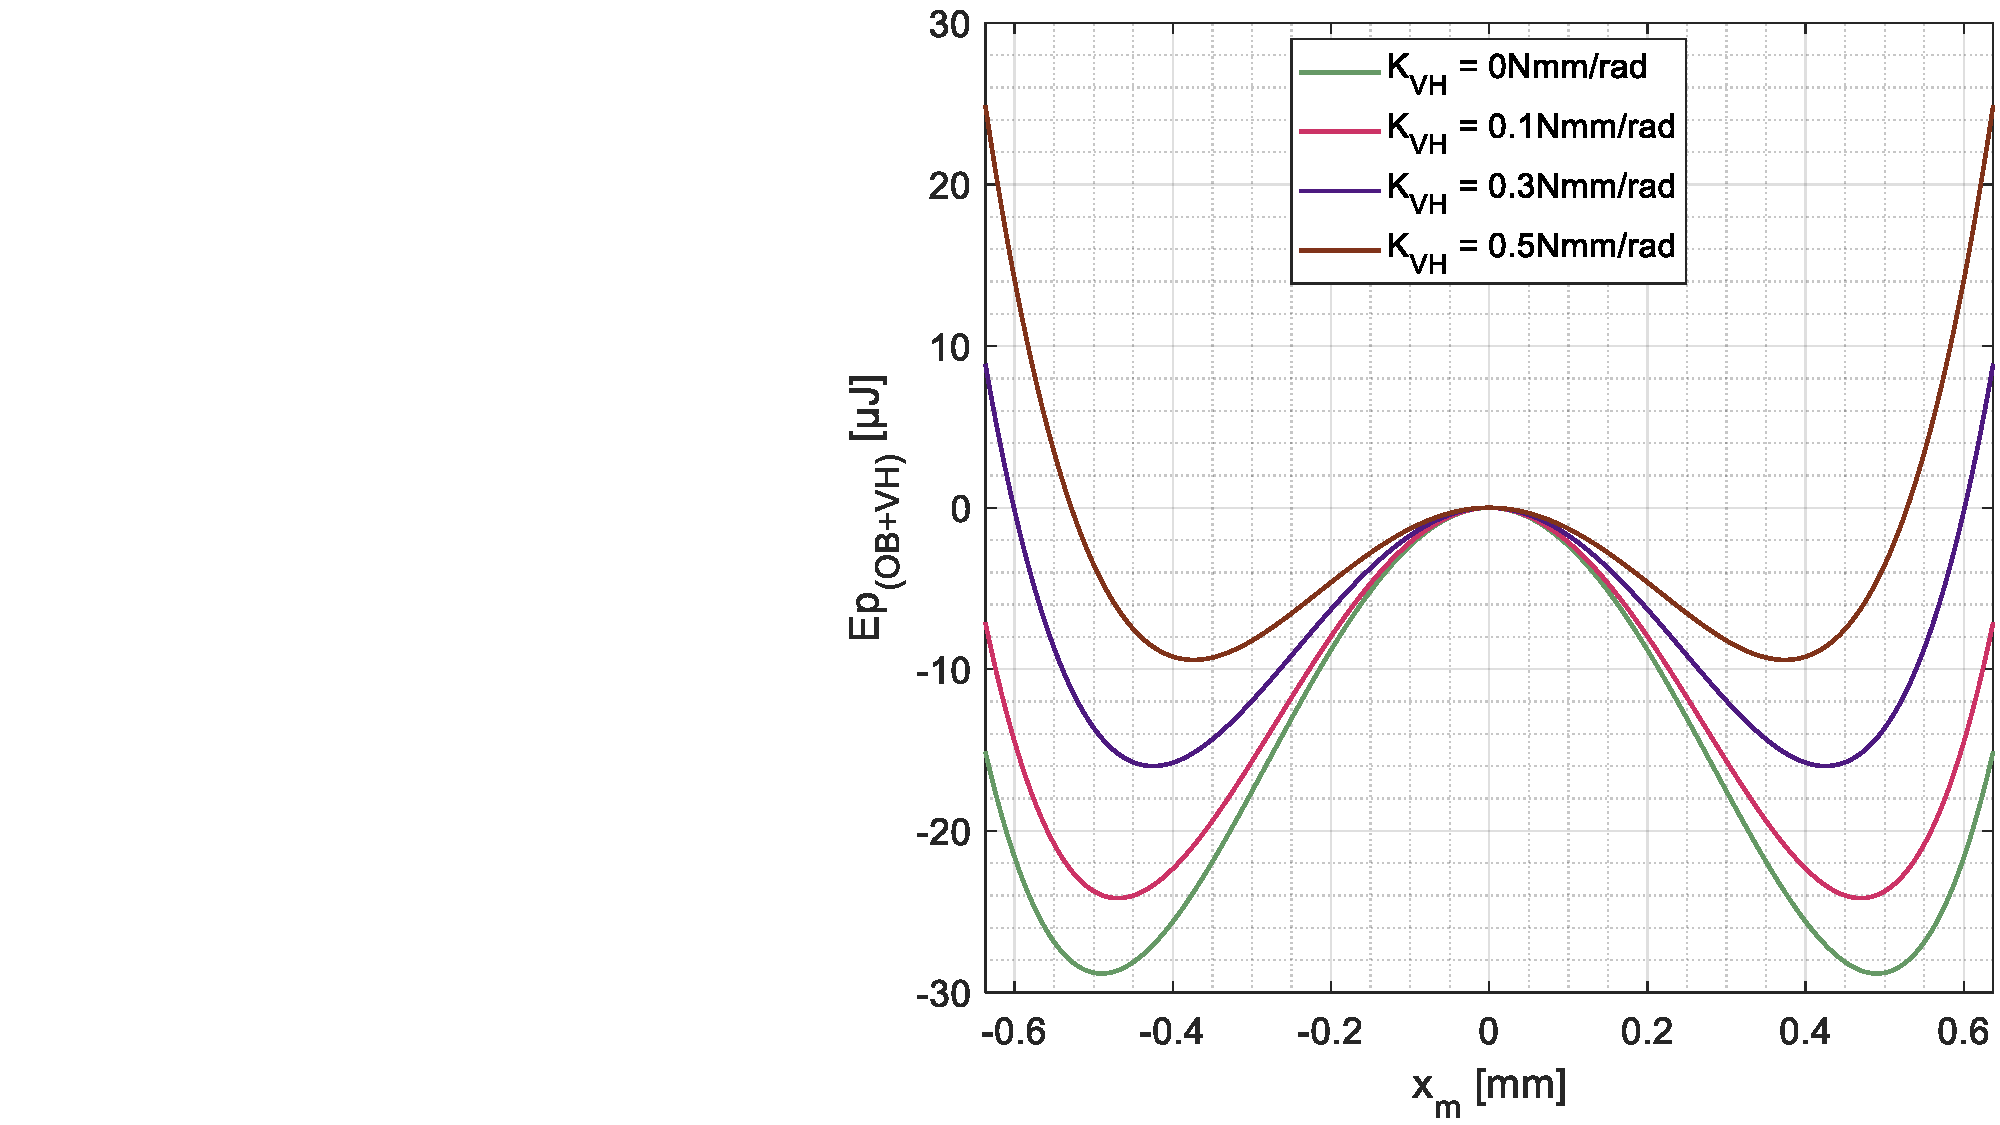
\includegraphics[trim={14cm 0cm 0cm 0cm},clip,width=0.6\textwidth]{../Chap5/Figure/(Ep)_vs_(x_m)_avec_plusieurs_K_VH.pdf}
		\caption{Impact de $K_{VH}$ sur le la tendance de l'évolution de l'énergie potentielle de M}
		\label{fig:(Ep)_vs_(x_m)_avec_plusieurs_K_VH}
	\end{center}
\end{figure}  
%%%%%%%%%%%%%%%%%%%%%%%%%%%%%%%%%%%%
La figure \ref{fig:(Ep)_vs_(x_m)_avec_plusieurs_K_VH} montre alors l'évolution de l'énergie potentielle de la masse M dans le système OBVH, pour différentes rigidités de tubes. La rigidité $K_{VH}$ du tube semble alors avoir un effet similaire à la rigidité $K_{\varphi}$ des liaisons pivot souples, comme le montre aussi la figure \ref{fig:Kphi_Ep}. Augmenter $K_{VH}$, pour un niveau de flambement fixe, a pour conséquence de ramener les positions d'équilibre stable de M vers l'axe $x=0$. On rappelle que l'énergie transmise par le PH à l'OBVH correspond à la différence d'énergie potentielle lorsque $x_m=0$ et $x_m=x_{0,vh}$, où $x_{0,vh}$ est la position d'équilibre finale de M sous l'influence de $K_{VH}$. La barrière énergétique, et par extension la force nécessaire pour passer d'une position stable à l'autre, diminue alors avec l'augmentation de $K_{VH}$. Du point de vue récupération, cela veut dire qu'en augmentant $K_{VH}$, l'énergie exploitable par le récupérateur diminue. En effet, l'énergie récupérée par cycle de mastication est une fraction de la barrière de potentiel à franchir par la masse M. En conséquence, même si le rendement reste inchangé, l'énergie récupérée pour un cycle de fermeture de mâchoire est d'autant plus faible que $K_{VH}$ augmente, pour un niveau de flambement considéré fixe.

Nous pouvons calculer la nouvelle position d'équilibre $x_{0,vh}$ du système OBVH, lorsque l'OB est flambé en $x_0$ et que la VH rentre ensuite en contact avec M. Cette position est définie par l'équation \ref{eq:x0_vh_statique} qui traduit l'équilibre statique du système OBVH.
\begin{equation}
\frac{2K\ {x_{0}}^2}{L^2}\biggl(\frac{{x_{0,vh}}^2}{{x_{0}}^2}-1\biggr)x_{0,vh}
\ +\ \frac{K_{VH}(x_m)}{a}\cdot \theta({x_m})
\ =\ 0 
\label{eq:x0_vh_statique}
\end{equation}

Pour relever la barrière énergétique de l'OBVH, il faudrait augmenter le niveau de flambement initial sur l'OB, en veillant à ce qu'il reste inférieur à $x_{0,m}$. On peut alors déterminer le niveau de flambement du système OBVH$_{eq}$ dont la barrière énergétique serait équivalente à celle d'un OB seul. Cela revient à dimensionner le nouveau niveau de flambement initial $x_{0,eq}$ à appliquer sur l'OB$_{eq}$ pour compenser $K_{VH}$. Cette méthode de redimensionnement est très pertinente dans le cas de figure où le niveau d'entrée énergétique est limité et connu. La barrière de potentiel du système OBVH$_{eq}$ peut alors être en permanence réglée de façon à être légèrement en dessous de l'apport d'énergie par le PH, et ainsi permettre de maximiser l'énergie récupérée.

Le système d'équations (\ref{eq:x0_eq_energetique}-\ref{eq:x0_eq_statique}) définit alors les critères de redimensionnement du système OBVH$_{eq}$.
\begin{subnumcases}{}
$$
\dfrac{K\ {x_{0,vh}}^2}{2L^2}
\biggl({x_{0,vh}}^2 - 2{x_{0,eq}}^2\biggr)+				
\bigint_{~0}^{x_{0,vh}} \dfrac{K_{VH}(x_m)}{a}\cdot \theta({x_m})\ dx_m\ 
=\ \dfrac{K\ {x_{0}}^4}{2L^2} 
$$
\label{eq:x0_eq_energetique}\\
%%%%%%%%%%%%%%%%%%%%
$$
\dfrac{2K\ {x_{0,eq}}^2}{L^2}\biggl(\dfrac{{x_{0,vh}}^2}{{x_{0,eq}}^2}-1\biggr)x_{0,vh}
\ +\ \dfrac{K_{VH}(x_m)}{a}\cdot \theta({x_m})
\ =\ 0
$$
\label{eq:x0_eq_statique}
\end{subnumcases} 

L'équation \ref{eq:x0_eq_energetique} traduit la contrainte d'égalité des barrières d'énergie potentielle entre l'OB et l'OBVH$_{eq}$. Enfin, l'équation \ref{eq:x0_eq_statique} traduit l'équilibre statique qui doit se produire quand $x_m=x_{0,vh}$. Enfin, la valeur du bras de levier de pliage $a$ peut être calculée à partir de la cinématique AG définie par les équations \ref{eq:f}-\ref{eq:x_0f}.

Les notations des différents systèmes établis peuvent se résumer par la suivante :
\begin{itemize}[label=$\circ$]
	\item \textbf{OB} : Oscillateur bistable seul flambé à $x_{0}$.
	\item \textbf{OBVH}: Système composé de l'OB en contact avec la VH.
	\item \textbf{OB$_{eq}$}: Oscillateur bistable seul flambé à $x_{0,eq}$.
	\item \textbf{OBVH$_{eq}$}: Système composé de OB$_{eq}$ en contact avec la VH.
\end{itemize}

Le système d'équations (\ref{eq:x0_eq_energetique}-\ref{eq:x0_eq_statique}) peut dans certains cas ne pas trouver de point de fonctionnement physique satisfaisant $\Delta\theta$ avec la cinématique AG. Une solution pragmatique est alors de fixer $x_{0,vh} = x_0$ dans le cahier des charges du système OBVH$_{eq}$ et de prendre en considération seulement la contrainte d'équilibre statique (éq. \ref{eq:x0_eq_statique}), en supposant qu'elle suffit aussi à remplir la contrainte d'égalité énergétique. La pertinence de ce choix peut être vérifiée en considérant le redimensionnement de l'OBVH avec les données expérimentales du tube T100p caractérisé dans le chapitre \ref{ch:4_Valves hydrauliques a base de tubes flexibles flambes}.

Par ailleurs, la nouvelle position critique $x_{c,eq}$ de M, où le piston rencontre une résistance maximale, peut être calculée à partir de l'équation \ref{eq:xc_vh_OU_xc_eq}.
\begin{equation}
\dfrac{2K}{L^2}\biggl(3{x_{c,eq}}^2-{x_{0,eq}}^2\biggr) \ 
+\ 
\frac{1}{a}\biggl( \dfrac{\text{d}K_{VH}}{\text{d}x_m}(x_{c,eq}) \cdot \theta(x_{c,eq}) + K_{VH}(x_{c,eq}) \cdot \dfrac{\text{d} \theta}{\text{d} x_m}(x_{c,eq}) \biggr)
\ =\ 0
\label{eq:xc_vh_OU_xc_eq}
\end{equation}

La force critique $F_{c,eq}$ pourra aussi être calculée, en évaluant l'expression de la force élastique de l'OBHV$_{eq}$ en $x_m=x_{c,eq}$. Elle s'exprime donc avec l'équation \ref{eq:new_Fcrit}.
\begin{equation}
F_{c,eq} = \frac{2K\ {x_{0,eq}}^2}{L^2}\biggl(\frac{{x_{c,eq}}^2}{{x_{0,eq}}^2}-1\biggr)x_{c,eq}
\ +\ 
\frac{K_{VH}(x_{c,eq})}{a}\cdot \theta({x_{c,eq}})
\label{eq:new_Fcrit}
\end{equation}

Il est important d'évaluer $F_{c,eq}$ afin de déterminer le niveau d'amplification hydraulique $a_h$ permettant de respecter la contrainte de confort exprimée au travers de l'équation \ref{eq:critere_confort}. Afin de s'affranchir de cette étape calculatoire, nécessitant les expressions des dérivées des fonctions non linéaires $K_{VH}$ et $\theta$ par rapport à $x_m$, il est possible de déterminer $x_{c,eq}$ et $F_{c,eq}$ par une approche numérique. Les données expérimentales permettent en effet d'évaluer $K_{VH}(x_m)$ et $\theta(x_m)$. L'allure de la force élastique de l'OBHV$_{eq}$ peut alors être obtenue par l'implémentation des relevés expérimentaux dans l'équation \ref{eq:x0_eq_statique}, pour $x_m\in[0;x_{0,vh}]$. La force critique $F_{c,eq}$ correspond alors au maximum de la courbe obtenue et $x_{c,eq}$ est son abscisse.
%%%%%%%%%%%%%%%%%%%%%%%%%%%%%%%%%%%%%%%%%
    %/////////////////////////////////////////////	
	\subsection{Redimensionnement du système sur critère énergétique}
	\label{subsec:6.1.2_Redimensionnement du systeme sur critere energetique}
    %/////////////////////////////////////////////	
% LTeX: language=fr
L'énergie potentielle pouvant être emmagasinée dans le récupérateur diminue sous l'influence de la raideur de la VH. Il est donc important de recaler les paramètres de l'OB afin d'adapter le système au niveau d'énergie d'entrée, dans le respect de la contrainte de confort (\ref{eq:critere_confort}). Avec la méthode de redimensionnement basée sur les équations introduites dans la section précédente, il est possible de recalculer les paramètres du système suite à l'intégration des données expérimentales de la VH composée du tube T100p. Le fonctionnement que doit cibler le système OBVH$_{eq}$ est celui issu des simulations corrélées aux données expérimentales de caractérisation de l'OB seul (tab. \ref{tab:parametres_lacher_free}). Voici les étapes à suivre afin de redimensionner le système sous l'influence de la VH :
\begin{itemize}[label=$\circ$]
	\item \textbf{Avant l'implémentation des influences statique et hydraulique de la VH :}
	      \begin{enumerate}
		      \item Calculer la position d'équilibre finale $x_0$ de l'OB imposée par la contrainte de confort définie à l'équation \ref{eq:critere_confort} et les éventuelles limites structurelles, se résumant ici par un niveau de flambement maximal admissible déterminé à l'équation \ref{x0_max}.
		      \item Réaliser les simulations itératives avec le modèle préliminaire sans tenir compte de l'influence de la VH. Cela se fait par la résolution numérique des équations définissant les phases de fonctionnement du système (sec. \ref{subsec:2.5.3:Simulation et resultats}). La valeur de $(r_{Cf})_{min}$ nécessaire pour assurer la bonne commutation des branches hydrauliques est alors déterminée à l'issue du processus itératif. Cela donne le CdC hydraulique de la VH et permet d'évaluer $\Delta\theta$ avec les données expérimentales du T100p. Ce dernier critère donne alors les évolutions respectives de $C_f(\theta)$ et $K_{VH}(\theta)$.
	      \end{enumerate}
\end{itemize}
\begin{itemize}[label=$\circ$]
	\item \textbf{Après l'implémentation des influences statique et hydraulique de la VH :}
	      \begin{enumerate}
		      \item Calculer le nouveau niveau de flambement $x_{0,eq}$ nécessaire à appliquer sur l'OB afin de compenser l'influence statique de la VH. Cela se fait au travers du système d'équations (\ref{eq:f}-\ref{eq:equilibre_statique}) en imposant $\Delta\theta$ et $x_{0,vh} = x_0$. Par la même, cela fixe la valeur du bras de levier de pliage $a$.
		      \item Trouver un point de fonctionnement optimal en faisant varier $\Delta\theta$ et en réitérant l'étape précédente. Cela se fait en considérant deux contraintes nécessitant un compromis :
		            \begin{itemize}[label=$\bullet$]
			            \item Minimiser l'angle d'ouverture $\theta_0$ pour limiter les dissipations hydrauliques dans la branche active et, par conséquent, maximiser le rendement. Cela induit aussi une réduction de $(r_{Cf})$ pour $\Delta\theta$ fixe.
			            \item Maximiser $\Delta\theta$ pour assurer $(r_{Cf})_{min}$. Cela induit aussi une réduction du bras de levier de pliage $a$ et augmente par conséquent l'influence de $K_{VH}$ sur l'OB.
		            \end{itemize}
	      \end{enumerate}
\end{itemize}	
% LTeX: language=fr
\begin{figure}[!htbp]
\begin{center}
		\captionsetup{justification=centering} 
		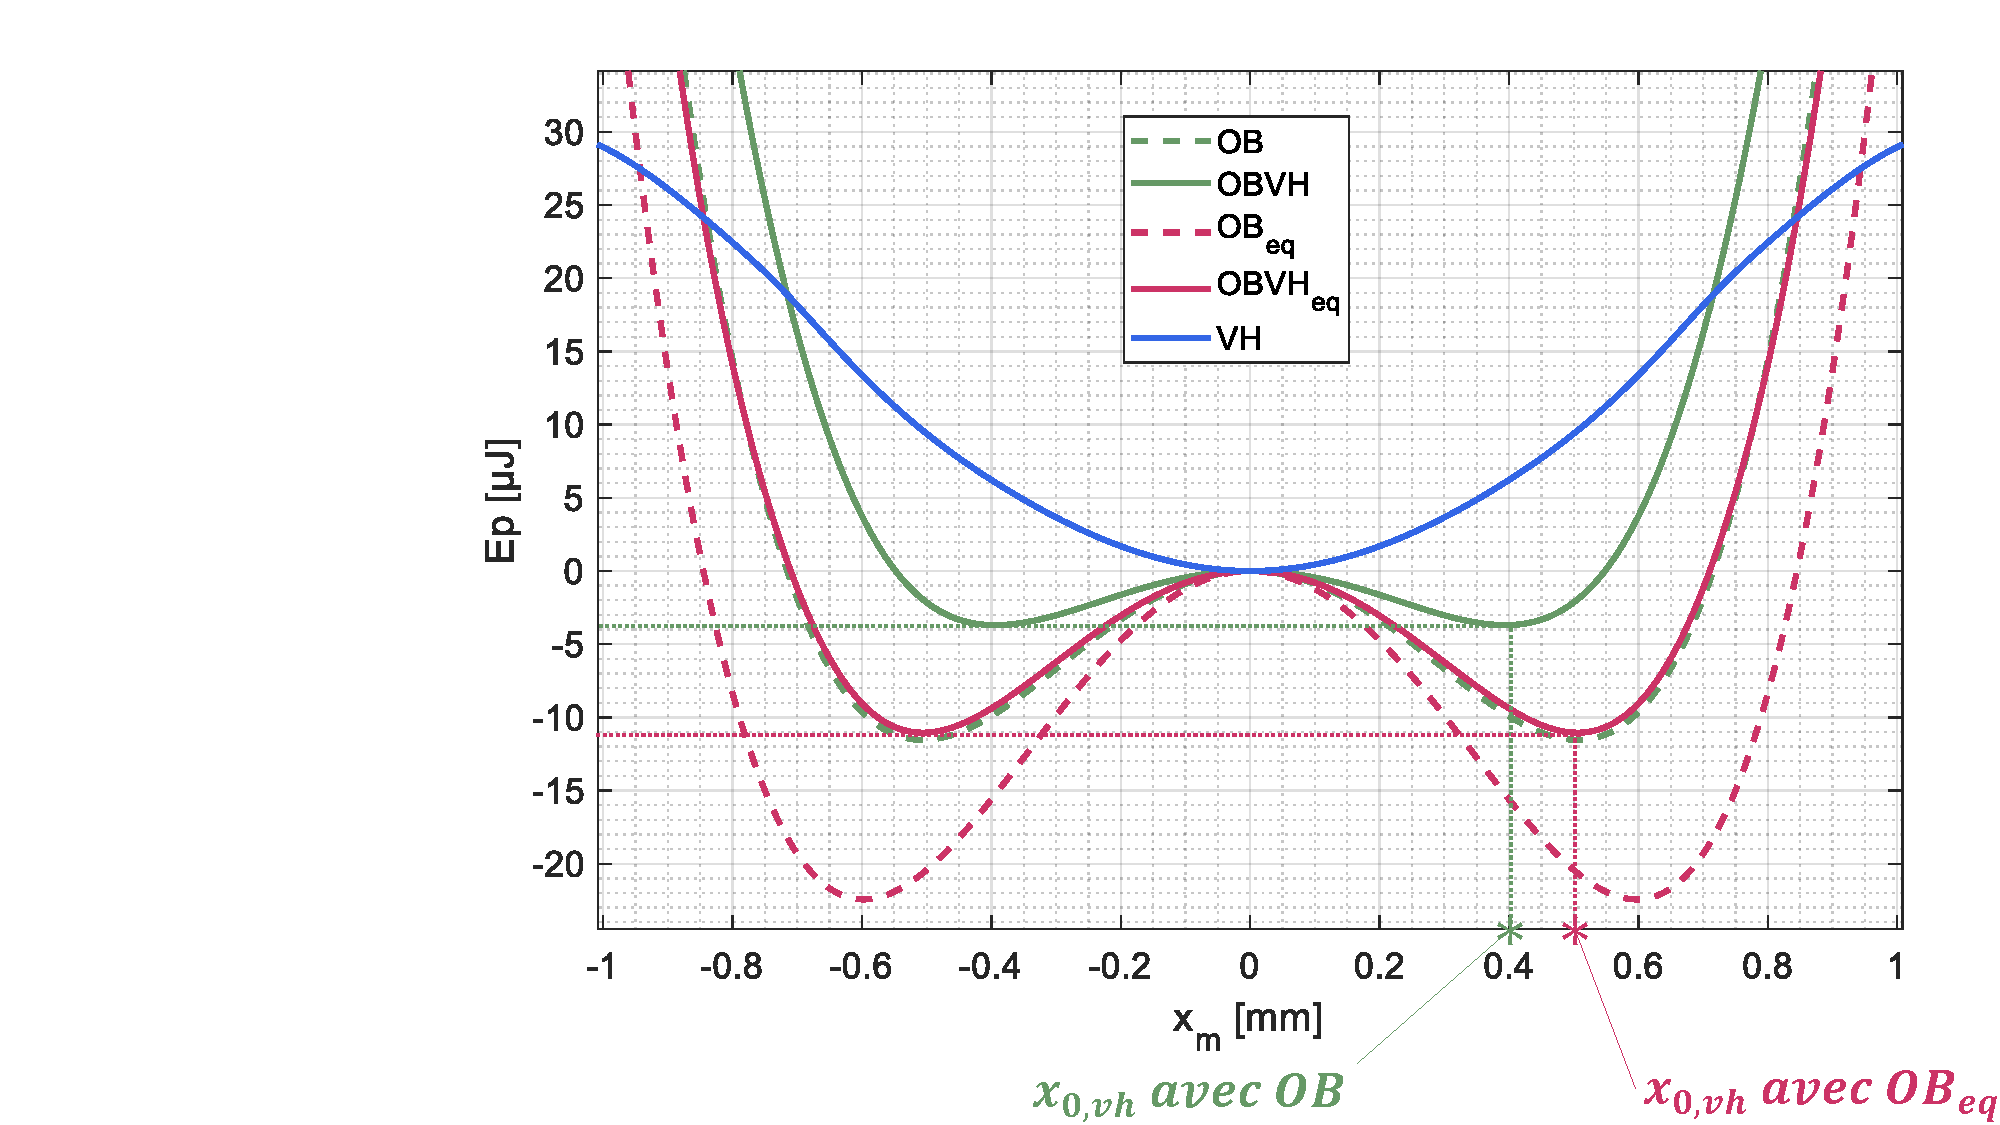
\includegraphics[trim={8cm 0cm 0cm 1cm},clip,width=0.8\textwidth]{../Chap6/Figure/Energie_potentielle_OBVHeq.pdf}
		\caption{Évolution de l'énergie potentielle dans les différents systèmes avec et sans VH}
		\label{fig:Evolution energie potentielle tous les systemes}
\end{center}	
\end{figure} 
%%%%%%%%%%%%%%%%%%%%%%%%%%%%%%%%%%%%%%%
\begin{table}[!htbp]
	\centering
	\rowcolors[]{2}{black!8}{}{
		\begin{tabular}[t]{c c}
		\rowcolor{blue!10}
\toprule
Paramètre & Valeur \\
\midrule
$x_{0,eq}$					&	0.60mm		\\ 
\textbf{$x_{0,vh}$}			&	0.50mm		\\ 
$a$							&	1.89mm 		\\
\textbf{$\theta_0$}			&	20deg		\\ 
\textbf{$\Delta\theta$}		&	45deg		\\ 
\textbf{$r_{Cf}$}			&	18.60		\\ 
\bottomrule
		\end{tabular}}
        \caption{Paramètres des système OBVH$_{eq}$ redimensionné}
        \label{tab:recalage_OBVH_xp}
\end{table}  
Le tableau \ref{tab:recalage_OBVH_xp} donne alors les valeurs des paramètres redimensionnés pour le système OBVH$_{eq}$ après les itérations des étapes explicitées ci-dessus. La figure \ref{fig:Evolution energie potentielle tous les systemes} montre par ailleurs l'évolution de l'énergie potentielle des systèmes définis précédemment, ainsi que celle de la VH.

Le seul critère d'équilibre statique en $x_{0,vh} = x_0$ suffit à compenser l'influence de $K_{VH}$ en rehaussant la valeur de la barrière d'énergie potentielle. De plus, la compensation se fait à un niveau de flambement $x_{0,eq} < x_{0,max}$ appliqué l'OB$_{eq}$, garantissant ainsi un meilleur coefficient de couplage électromécanique sur le prototype fabriqué (tab. \ref{tab:x0max}). La corrélation n'est pas exacte avec l'OB, car l'évolution de $K_{VH}(x_m)$ n'est pas linéaire. Néanmoins, cela n'influe pas de façon significative sur l'évolution de la barrière de potentiel du système OBVH$_{eq}$ pour une position $x_{0,vh}$ donnée. Elle peut donc être approximée à celle d'un OB seul flambé à $x_{0,vh}$, s'exprimant par l'équation \ref{eq:Eb_OB}.
\begin{equation}
	Eb_{OBVH_{eq}} = Eb_{OB} = \dfrac{ K {x_{0,vh}}^4 }{ 2L^2 }
	\label{eq:Eb_OB}
\end{equation}
%/!\/!\/!\/!\/!\/!\/!\/!\/!\/!\/!\/!\/!\/!\/!\/!\/!\/!\/!\/!\/!\/!\/!\/!\	
\section{Implémentation du frottement au contact M-VH au modèle système}
\label{subsec:4.3.4_Implementation du frottement au contact M-VH au modele systeme}
%/!\/!\/!\/!\/!\/!\/!\/!\/!\/!\/!\/!\/!\/!\/!\/!\/!\/!\/!\/!\/!\/!\/!\/!\
    %///////////////////////////////////////////// 	
	\subsection{Essais de lâchers experimentaux de M avec et sans VH}
	\label{subsec:6.2.2_Essais de lacher experimentaux de M avec et sans VH}
    %///////////////////////////////////////////// 
Les résultats des essais présentés dans cette sous-section sont obtenus grâce au banc d'essai présenté pour la mise en évidence de l'évolution de la cinématique de pliage suite à l'influence du diamètre de la GR (fig \ref{fig:presentation_BDT_lacher_tube}).\\	
Pour caractériser les pertes énergétiques par frottement au contact M-VH, on se place dans la configuration la plus proche du système OBVH$_{eq}$ dont les paramètres sont donnés dans le tableau \ref{tab:recalage_OBVH_xp}. Les paramètres de réglage sont choisis en fonction de la précision des moyens mis en \oe{}uvre à cet effet. Par conséquent, la position d'équilibre finale $x_{0,vh}$ du système OBVH est réglée grâce à la mesure de la position de M par le capteur laser, ainsi que grâce à la vis micrométrique qu'on retrouve sur la figure \ref{fig:BDT_OB+GPA}. Ensuite, l'aspect important à régler est la plage d'angle $\Delta\theta$ pour satisfaire le CdC du fonctionnement de la VH. Expérimentalement, il est plus simple de régler $a$ de façon qualitative à 2mm (tab. \ref{tab:recalage_OBVH_xp}) et déduire $\Delta\theta$ avec les positions de M avant et après le contact M-VH (fig. \ref{fig:BDT_OB+GPA}). Ce réglage peut être itératif de façon à obtenir le $\Delta\theta$ souhaité. La raideur $K_{T100p}(\theta_f)$ peut alors être extraite des essais statiques réalisés sur le tube considéré.  
%%%%%%%%%%%%%%%%%%%%%%%%%%%%%%%%%%%%	
\begin{figure}[!htbp]
	\begin{center}
		\captionsetup{justification=centering}
		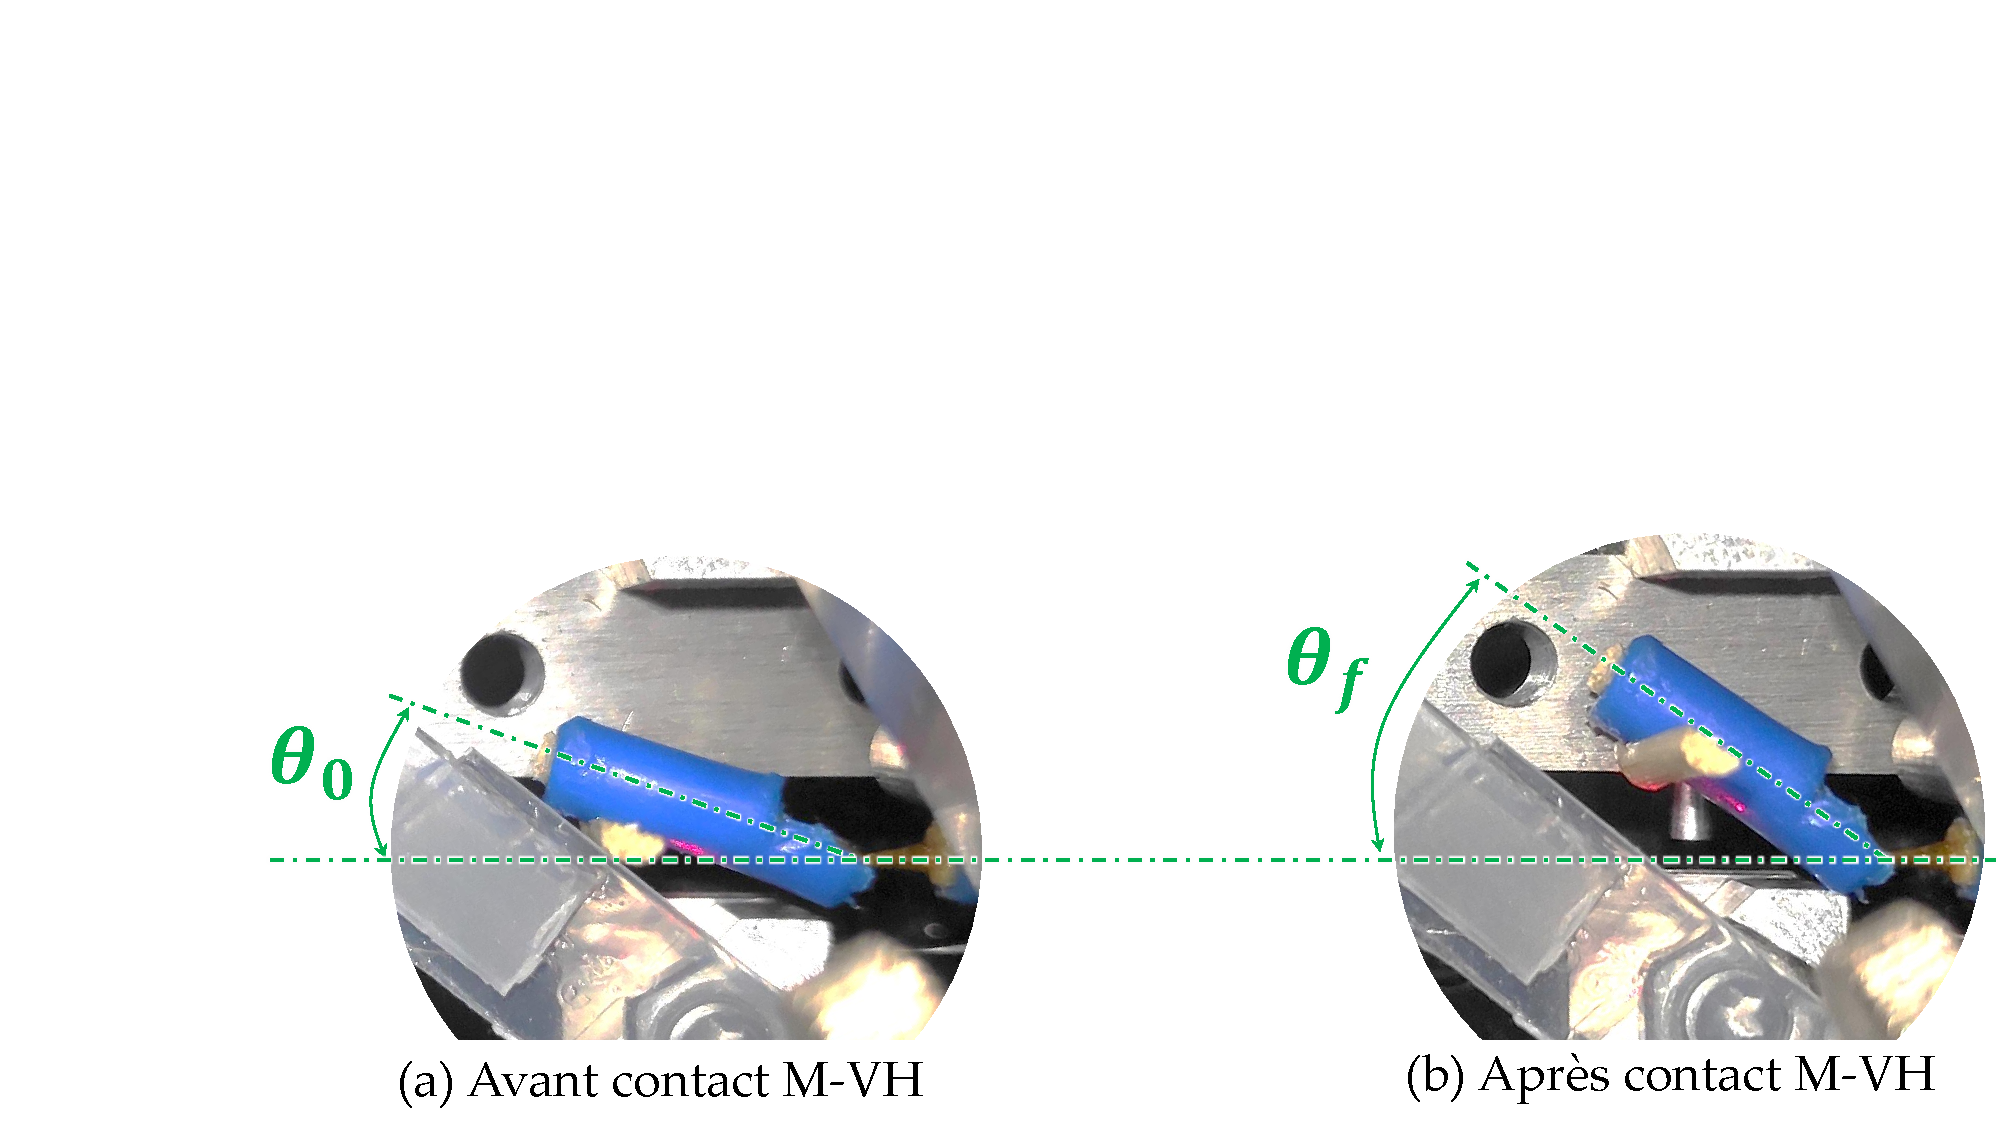
\includegraphics[trim={4cm 0cm 0cm 9.5cm},clip,width=0.8\textwidth]{../Chap6/Figure/contact_M_VH_lachers.pdf}
		\caption{Image de la VH$_{T100p}$ lorsque $\theta_0$($x_m=-x_{0})$ et lorsque $\theta_f$($x_m=x_{0,vh}$)}
		\label{fig:contact_M_VH_lachers}
	\end{center}
\end{figure}
%%%%%%%%%%%%%%%%%%%%%%%%%%%%%%%%%%%%

Le tube n'est présent que du côté où on considère $x_m$ positif. La masse M se trouve alors à l'équilibre en $-x_{0}$ avant le contact et en $x_{0,vh}$ après que le contact ait été engagé. Un plan plus large du banc a été présenté sur la figure \ref{fig:presentation_BDT_lacher_tube} pour avoir plus de visibilité sur les composants environnants. Les essais de lâchers dont les résultats sont présentés sur la figure \ref{fig:lacher_avec et sans T100p} ont été réalisés suivant le protocole décrit dans la sous-section \ref{subsec:4.3.1_Presentation du banc de test}. Le déroulement des tests consiste à pousser la masse depuis $x_m=-x_0$ jusqu'à $x_m=0$ et la laisser osciller avec la VH jusqu'à son arrêt en $x_m=x_{0,vh}$. Dans un premier temps, les mesures sont effectuées avec la présence de la VH puis, dans un second temps, la VH est retirée, de façon à ce que le niveau de flambement initial sur l'OB reste identique. Le protocole des essais de lâchers est alors répété sur l'OB seul à titre de comparaison.

On retrouve dans le tableau \ref{tab:parametres lacher tube} les résultats de corrélation modèle-essais suite aux tests de lâchers illustrés sur la figure \ref{fig:lacher_avec et sans T100p}. Les valeurs des paramètres indiqués en rouge dans ce même tableau sont ceux qui ont été fixés et le reste des paramètres a été calculé d'après les équations régissant le modèle. Le recalage entre les données expérimentales et le modèle simulé a été fait sur l'amplitude des signaux de position $x_m$ et de tension $U_p$, ainsi que la fréquence d'oscillation naturelle du système OB ou OBVH considéré. La vitesse initiale $v_0$ des lâchers est prise en considération dans les simulations et sa valeur est extraite des données expérimentales. Le réglage de $\Delta\theta$ est réalisé manuellement avec une précision estimée à $\pm$\ang{2} à partir des images présentées sur la figure \ref{fig:contact_M_VH_lachers}.
%%%%%%%%%%%%%%%%%%%%%%%%%
\begin{figure}[!htb]
\begin{center}
	\begin{subfigure}[b]{0.49\textwidth}
    	\captionsetup{justification=centering}
		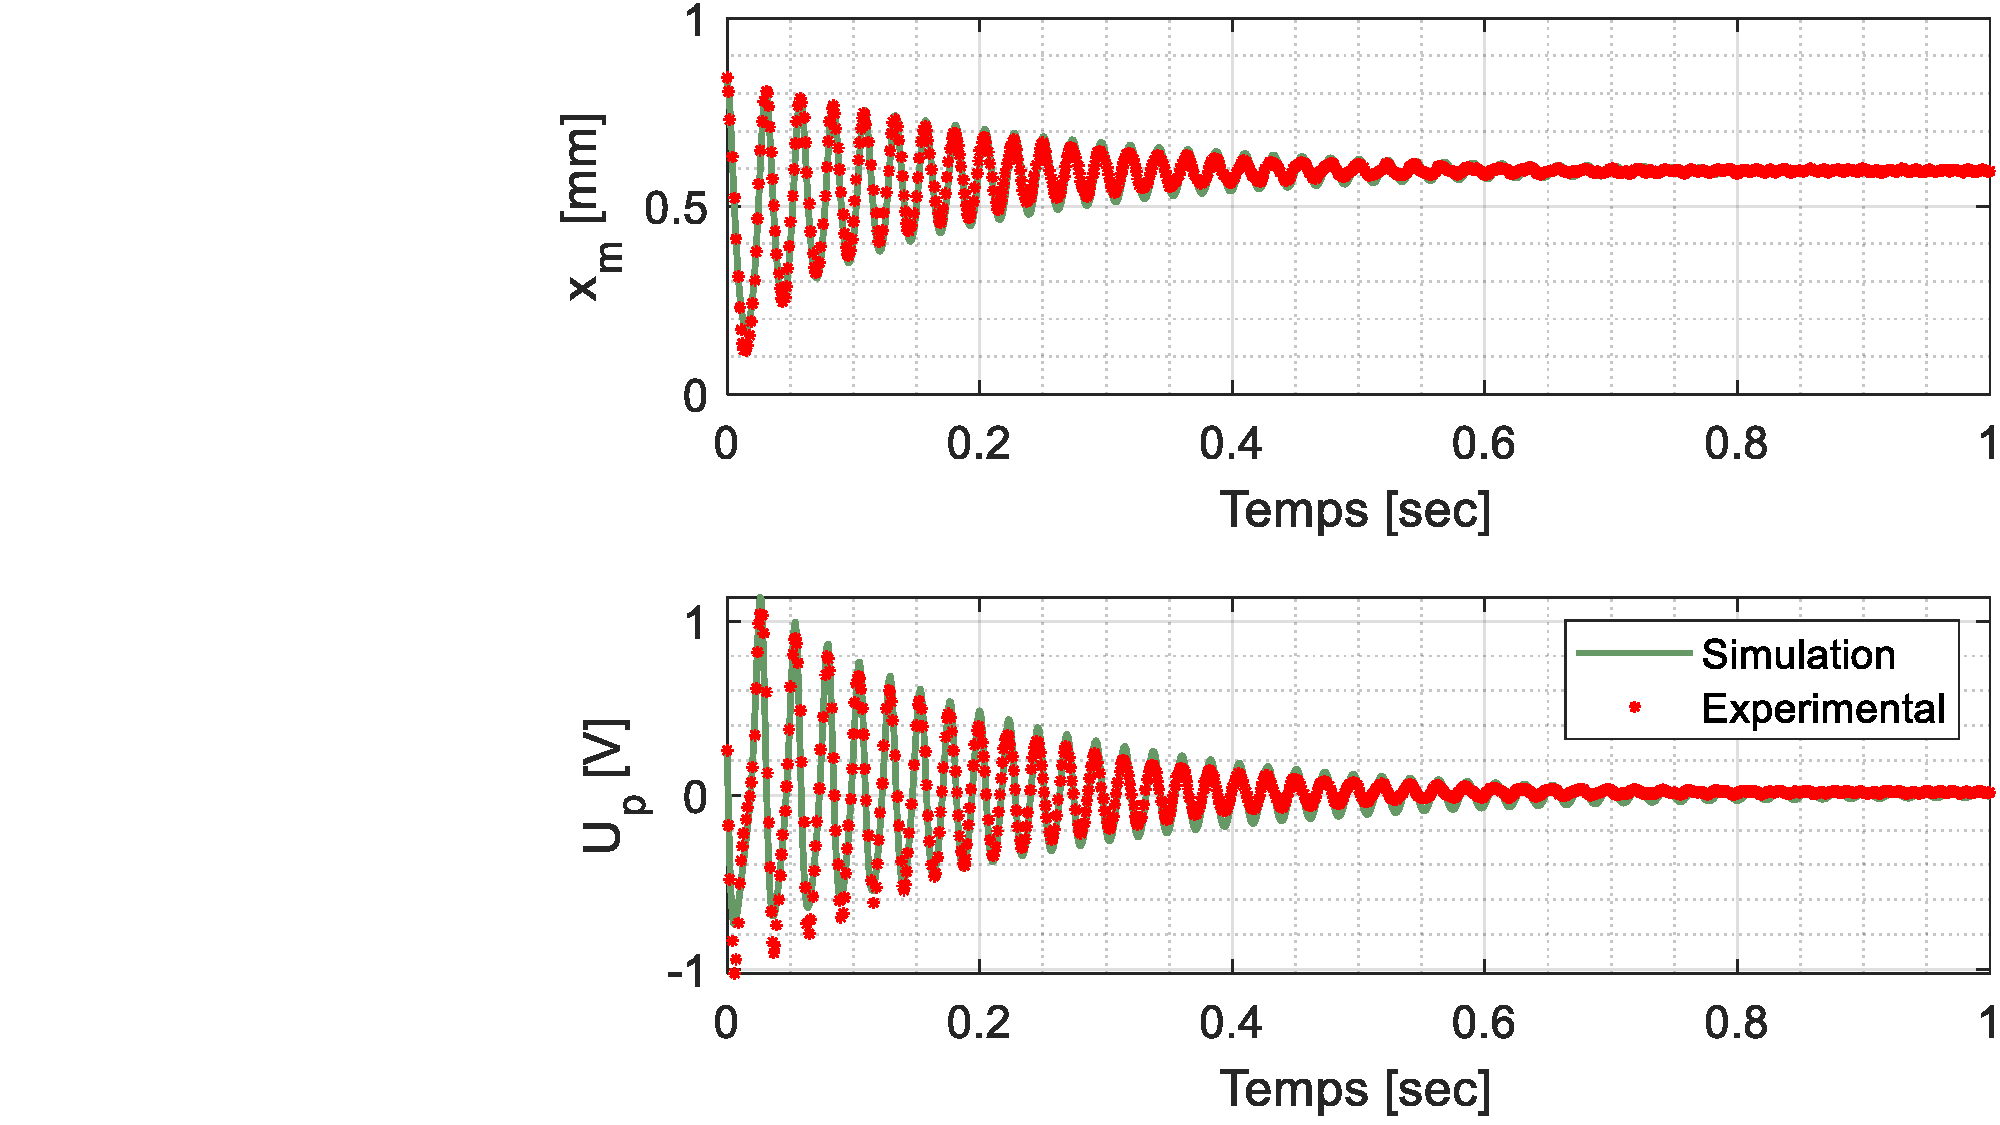
\includegraphics[trim={9cm 0cm 0cm 0cm},clip,width=\textwidth]{../Chap6/Figure/exp_lacher_free.pdf}
		\caption{Essais de lâcher sans VH}
		\label{fig:exp_lacher_free}
	\end{subfigure}
\hfillx
	\begin{subfigure}[b]{0.49\textwidth}
    	\captionsetup{justification=centering}
		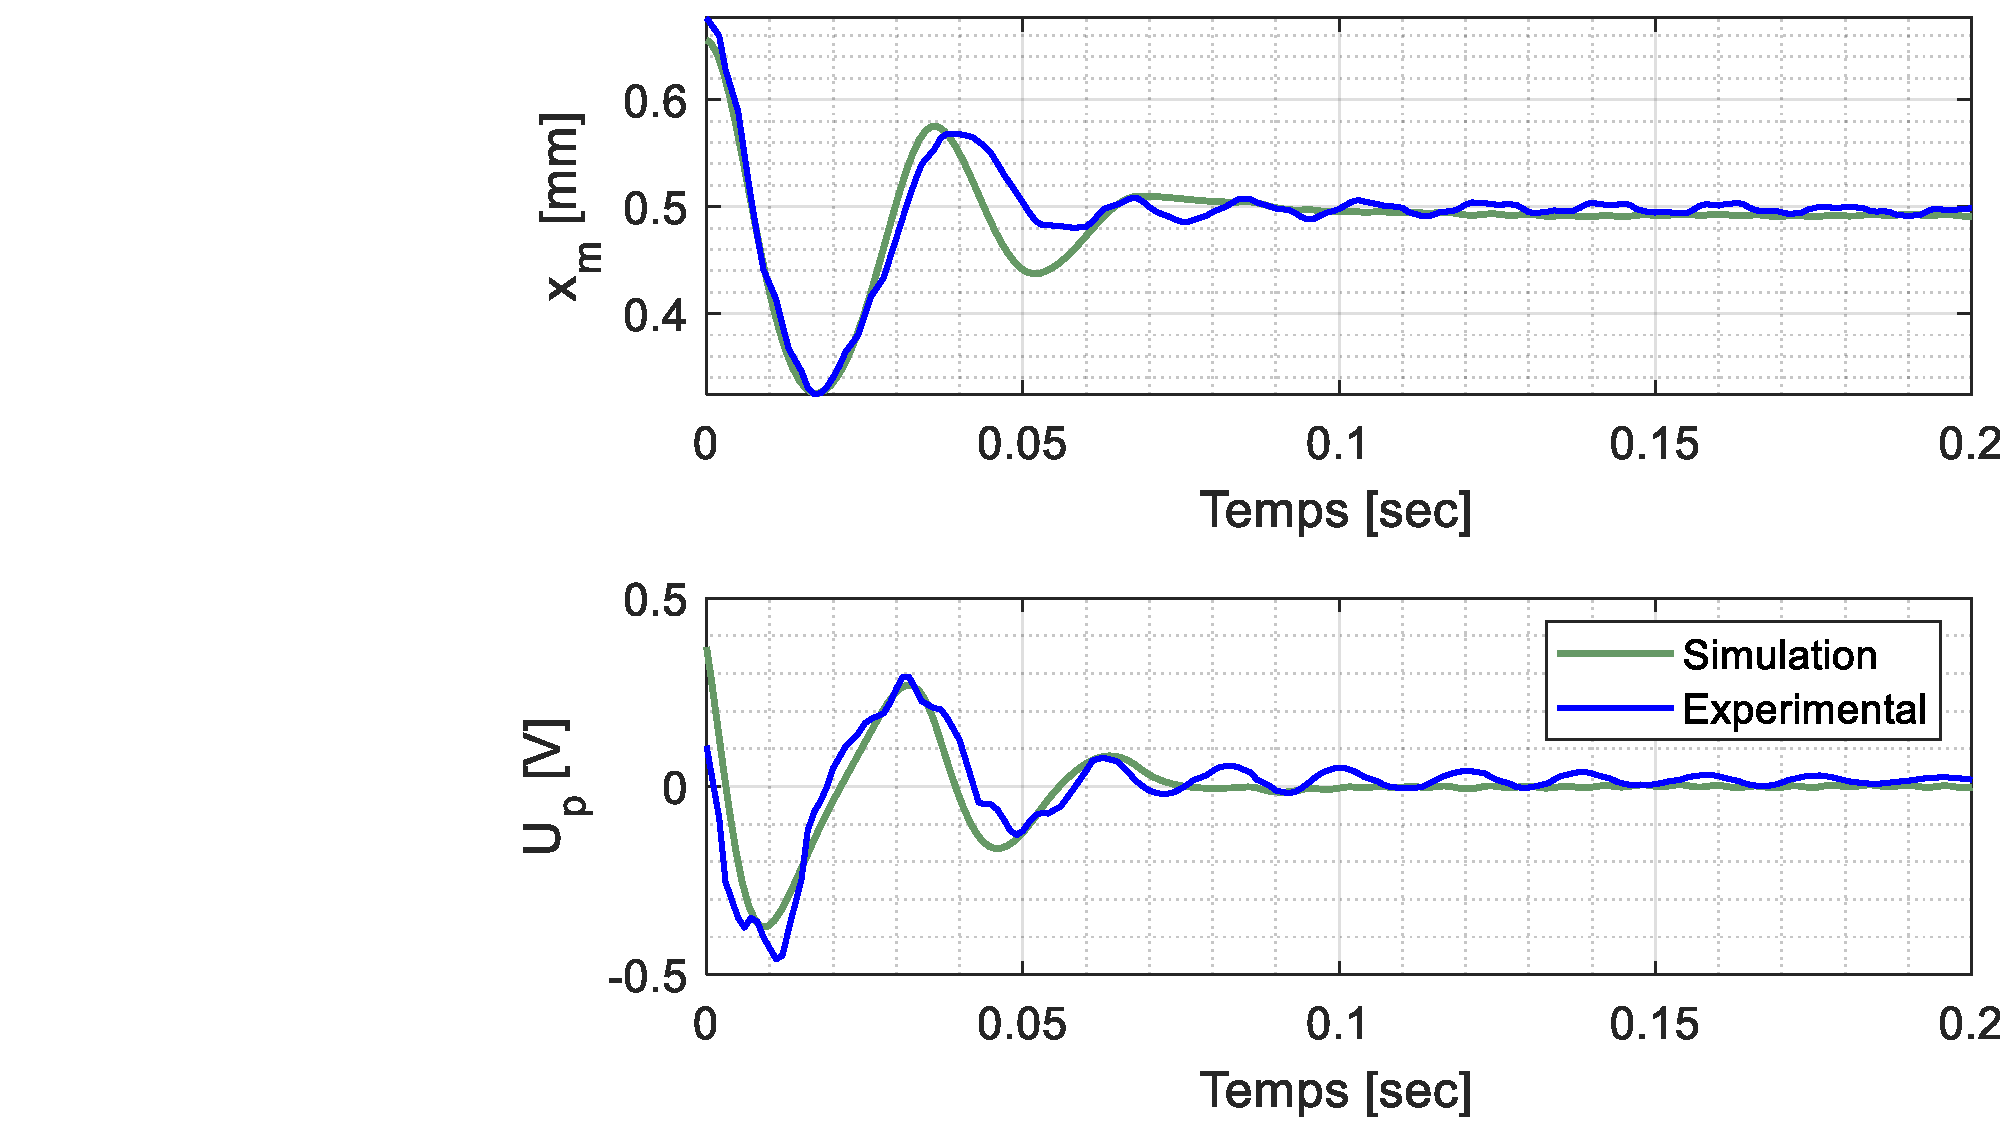
\includegraphics[trim={9cm 0cm 0cm 0cm},clip,width=\textwidth]{../Chap6/Figure/exp_lacher_t100p.pdf}
		\caption{Essais de lâcher avec VH$_{T100p}$}
		\label{fig:exp_lacher_t100p}  
	\end{subfigure}
	\caption{Corrélation modèle essais des essais de lâchers avec et sans la VH fabriquée à base du tube T100p}
	\label{fig:lacher_avec et sans T100p}
\end{center}	
\end{figure} 
%%%%%%%%%%%%%%%% 

Après la fabrication et la mise en place du système OBVH, on s'aperçoit qu'on se trouve dans le cas de figure où $b>0$ (fig. \ref{fig:(theta&a)_vs_xm_avec_et_sans_gaine_tot}). En nous référant à la figure \ref{fig:theta_vs_xm_avec_et_sans_gaine_tot}, on sait que si $b$ augmente, le passage du contact latéral supérieur, changeant la cinématique de pliage, a lieu pour des angles d'autant plus faibles. Les corrélations modèle-essais montrent cependant que $2a>D_{GR}$, ce qui veut dire que le contact M-VH reste latéral quel que soit $x_m$. 

La faible précision de la découpe de la GR, couplée à la complexité de la mise et du maintien en position de la VH sur le banc de test, rendent difficile le respect du CdC sur $\Delta\theta$. Notons ici qu'il est possible de régler les données dans le modèle numérique afin de simuler un comportement théorique avec les conditions initiales les plus proches du montage expérimental pour établir une corrélation modèle-essais pertinente. 

%%%%%%%%%%%%%%%%%%%%%%%%%%%%%%%%%%%
\begin{table}[!htbp]
	\centering
		\begin{tabular}[t]{|c|c|c|}
\hline
\textbf{Paramètre} & \textbf{Valeur OB} & \textbf{Valeur OBVH}  \\
\hline \hline
$D_g$ [mm] 						& \cellcolor{gray!30} 		& \textcolor{red}{4} 		\\ \hline
$\Delta\theta$ [deg] 			& \cellcolor{gray!30} 		& \textcolor{red}{{[$\approx$ 19 ; $\approx$ 36]}} \\ \hline
$K_{T100p}(\theta_f)$ [Nmm/rad] & \cellcolor{gray!30}  		&  0.27 					\\ \hline
$a$ [mm]         			    & \cellcolor{gray!30}  		&  2.24				 	 	\\ \hline
$\mu_{fs}$ [~~] 				& \cellcolor{gray!30}  		&  0.42  					\\ \hline
$K$ [N/m] 						&	84480			  	 	&  84480  					\\ \hline
$x_0$ [mm] 						& \textcolor{red}{0.59}		& \textcolor{red}{0.50}  	\\ \hline
$v_0$ [mm/s] 					& \textcolor{red}{10}		& \textcolor{red}{65}  		\\ \hline
$Q$	[~~] 						& 		24.0		 		& 5.0     					\\ \hline
$k^2_{sys}$ [\%] 						& 		1.25		 		& \textcolor{red}{1.25}   	\\ \hline
$\eta_{ob}$ [\%] 					& 		11.9		 		& 2.6   					\\ \hline	
$R_{ch}$ [k$\text{\ohm}$] 		&	\textcolor{red}{15.5}	& \textcolor{red}{15.5}    	\\ \hline		
$m$	[g]						    &	\textcolor{red}{5.88}	& 9.00   					\\ \hline	
$f_0$ [Hz]						&		32.9				& 27.9   					\\ \hline	
	\end{tabular}
        \caption{Valeur des paramètres de l'OB et de l'ensemble OBVH implémentant le tube T100p suite au essais de lâchers expérimentaux}
        \label{tab:parametres lacher tube}
\end{table}        
%%%%%%%%%%%%%%%%%%%%%%%%%%%%%%%%%%%%	
Un modèle de frottement sec est introduit dans le modèle de l'OBVH pour quantifier la dissipation mécanique au contact M-VH. Le coefficient de frottement $\mu_{fs}$ résultant s'ajoute alors aux degrés de liberté du recalage des données expérimentales avec les données simulées. Il est associé à la force de frottement $F_{fs}$ qui peut alors s'exprimer à travers l'équation \ref{eq:frotemment M-VH}.
\begin{equation}
	F_{fs} = \ \frac{\mu_{fs}\ K_{VH}\ \theta}{a\ \cos(\theta)}\ \sign(\dot{x}_m)
	\label{eq:frotemment M-VH}
\end{equation}

$F_{fs}$ peut être intégré dans le modèle de comportement dynamique, précédemment exprimé à l'équation \ref{eq:OB+GPA+VH+piston}, pour établir l'équation \ref{eq:OBVH avec frottements secs} qui prend en compte la nature du contact M-VH.
\begin{equation}
\ddot{x} = - \frac{K\ {x_0}^2}{m\ L^2}\biggl(\frac{{x_m}^2}{{x_0}^2} 
-1\biggr)\ x_m - \frac{\mu}{m}\ \dot{x}_m - \frac{\alpha\ U_p}{m\ L}\ \dot{x}_m - \frac{K_{VH}}{a}\ \theta - F_{fs}
\label{eq:OBVH avec frottements secs}
\end{equation}

L'essai de lâcher avec la VH est modélisé par l'OB en oscillation libre (éq. \ref{eq:x0_eq_statique}) sous l'influence de la raideur du tube, du frottement au contact M-VH et de la condition initiale $v_0$ sur la vitesse de départ. Le frottement sec au contact M-VH devrait alors induire un décalage sur la position finale de M. Pour mettre ce phénomène en évidence, nous avons réalisé deux simulations dont l'une avec $\mu_{fs}=0.42$ (tab. \ref{tab:parametres lacher tube}) et l'autre sans frottement sec. La différence de position finale entre les deux simulations est de $\Delta x_{0,vh}=0.01mm$. Cette dernière est de ce fait négligeable devant l'amplitude des oscillations. Elle est, de surcroît, difficilement repérable sur les résultats expérimentaux, car la précision des mesures du capteur laser est estimée à $\pm0.01mm$.
    %///////////////////////////////////////////// 	
	\subsection{Analyse et discussion}
	\label{subsec:6.2.2_Analyse et discussion}
    %///////////////////////////////////////////// 
L'évolution de $\theta(x_m)$ est régie par le système d'équations cinématiques avec gaine rigide, établi dans la sous-section \ref{subsec:4.3.2_Evolution de la cinematique d'actionnement}. Nous avons montré que lorsque $h$ (éq. \ref{eq:f}) tendait vers 0, la configuration de contact M-VH passait du latéral au supérieur. Or, d'après la figure \ref{fig:theta_saut_experimental} établie avec les données du tableau \ref{tab:parametres lacher tube}, $h$ admet une asymptote supérieure à 0 et donc le contact reste latéral quelle que soit $x_m$. Cela se produit lorsque le réglage du bras de levier de pliage est tel que $2a>Dg$. Ce cas de figure induit néanmoins une influence énergétique moins importante sur l'OB, car $a$ reste tout de même plus grand en comparaison avec une architecture de pliage sans GR.
 %%%%%%%%%%%%%%%%%%%%%%%%%
\begin{figure}[!htb]
	\begin{center}
		\begin{subfigure}[b]{0.49\textwidth}
			\captionsetup{justification=centering}
			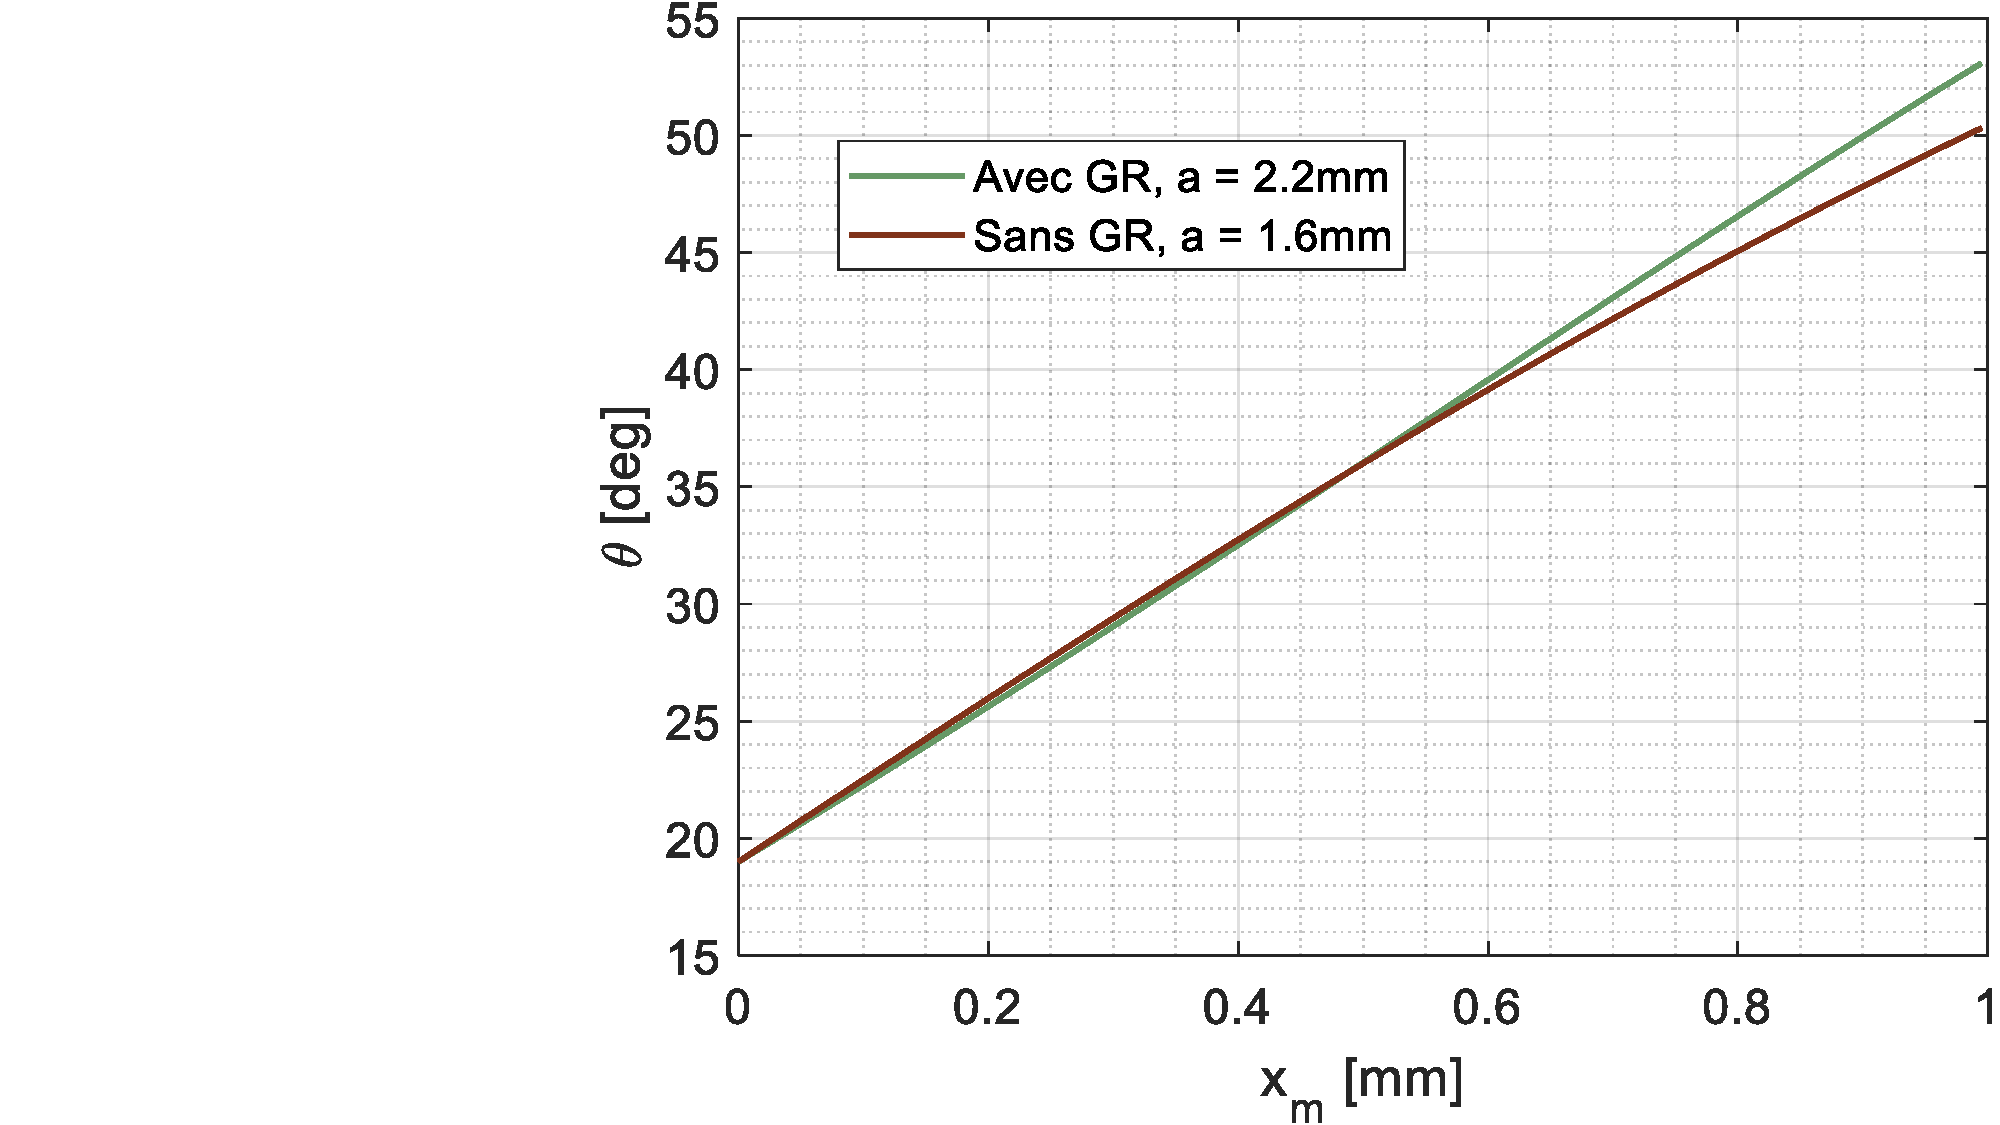
\includegraphics[trim={10cm 0cm 0cm 0cm},clip,width=\textwidth]{../Chap6/Figure/theta_vs_xm_avec_et_sans_gaine_experimental.pdf}
			\caption{Évolution de $\theta$ en fonction de $x_m$ avec recalage expérimental}
			\label{fig:theta_vs_xm_avec_et_sans_gaine_experimental}
		\end{subfigure}
		\hfillx
		\begin{subfigure}[b]{0.5\textwidth}
			\captionsetup{justification=centering}
			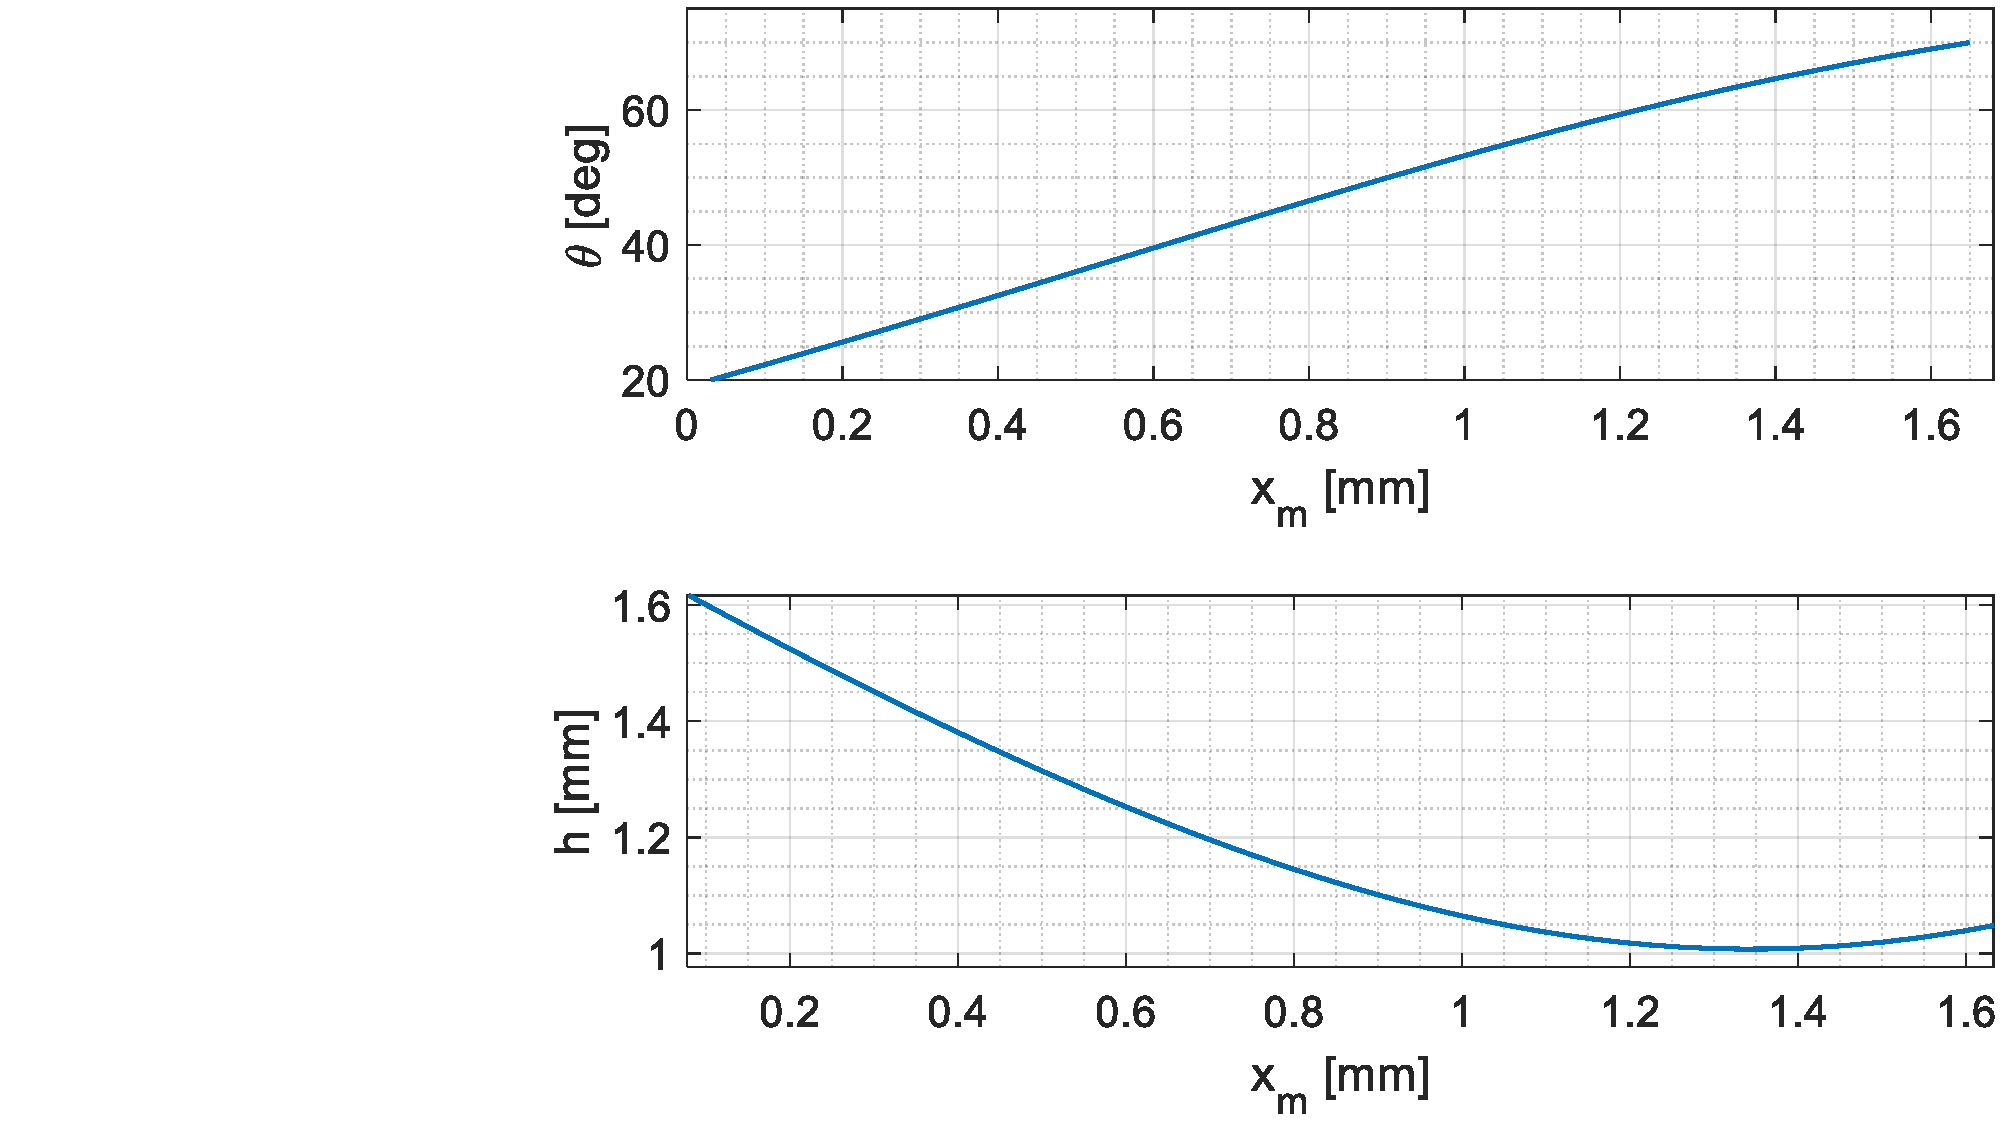
\includegraphics[trim={9cm 0cm 0cm 0cm},clip,width=\textwidth]{../Chap6/Figure/theta_saut_experimental.pdf}
			\caption{Évolution de $h$ et $\theta$ en fonction de $x_m$ lorsque $h$ tend vers 0, avec recalage expérimental}
			\label{fig:theta_saut_experimental}
		\end{subfigure}
		\caption{Corrélation modèle essais de la cinématique de pliage de la VH$_{T100p}$}
		\label{fig:Corrélation modèle cinématique VH}
	\end{center}
\end{figure}
%%%%%%%%%%%%%%%% 

D'autre part, en confrontant les données expérimentales avec et sans VH, on s'aperçoit de son impact sur la dynamique du système au travers de plusieurs aspects :
\begin{itemize}[label=$\bullet$]
	\item La valeur de $K_{T100p}(\theta_f)$ est extraite de l'équilibre des forces statiques exprimées par l'équation \ref{eq:equilibre_statique}. Elle est alors estimée à 40\% plus élevée que celle extraite des essais de caractérisation statique du tube T100p (fig. \ref{fig:(K_VH)_vs_theta_D1mm_plastifie}). Cette différence peut s'expliquer notamment par la faible répétabilité du processus de plastification locale réalisée à la main. Cette raideur reste néanmoins acceptable pour le niveau de flambement maximal $x_{0,max}$ de l'OB.
	\item Le contact M-VH étant permanent lors des oscillations, la masse dynamique se trouve augmentée de 50\% et donc la fréquence naturelle du système  OBVH se trouve réduite de 32\% car inversement proportionnelle à la racine carrée de $m$ (éq.\ref{eq:w0_Q}).
	\item Le facteur de qualité $Q$ est divisé par 5 suite à l'influence de la VH. Cela résulte des dissipations énergétiques supplémentaires apportées par l'intégration de la VH.\\
	Nous supposons que l'articulation au point $O$ se définit seulement par sa raideur en rotation. En revanche, nous n'avons pas intégré dans le modèle prédictif l'amortissement structurel du kapton lorsque celui-ci est soumis à des contraintes. Une partie de l'énergie servant à plier la VH est ainsi perdue par dissipation tout au long du mouvement de la VH.\\
	Le contact M-VH est de type quasi ponctuel entre un angle saillant en acier et un cylindre en polymère avec un état de surface rugueux. Le coefficient de frottement a alors été estimé dans le tableau \ref{tab:parametres lacher tube} en faisant la corrélation modèle-essais des tests de lâcher avec VH. Les dissipations énergétiques qui n'ont pas été prises en compte dans le modèle induisent alors une réduction de 94\% sur le rendement de l'OBVH. Les valeurs de rendement apparaissant dans le tableau \ref{tab:parametres lacher tube} prennent exclusivement en compte des pertes mécaniques lors des oscillations de la masse afin d'isoler les effets de frottement au contact M-VH. Les aspects de rendement énergétique du système dans sa globalité sont discutés dans la section qui suit.
\end{itemize} 	 
%/!\/!\/!\/!\/!\/!\/!\/!\/!\/!\/!\/!\/!\/!\/!\/!\/!\/!\/!\/!\/!\/!\/!\/!\
\section{Influence des différents paramètres sur le fonctionnement et l'efficacité du système global}
\label{subsec:6.3_Influence des differents parametres sur le fonctionnement et l efficacite du systeme global}
%/!\/!\/!\/!\/!\/!\/!\/!\/!\/!\/!\/!\/!\/!\/!\/!\/!\/!\/!\/!\/!\/!\/!\/!\
% LTeX: language=fr
Le système de récupération d'énergie est défini par de nombreux paramètres multiphysiques dimensionnés à partir de deux informations caractérisant la source : la pression de confort $p_c$ et la cylindrée $(\Delta V_{ear})_{max}$ du bouchon d'oreille. Pour le dimensionnement, l'allure du débit est supposée connue et imposée (fig. \ref{fig:debit_ear}). Il est alors possible, avec les résultats obtenus en sortie du modèle numérique, d'établir la tendance de l'évolution du système en fonction de la variation des paramètres de dimensionnement. Le tableau \ref{tab:influence parametres} présente un résumé de l'influence de chacun des paramètres sur le système en s'appuyant sur la maximisation de deux critères : rendement ($\tilde{\eta}$) et fonctionnement ($\tilde{f}$). $\tilde{\eta}$ se réfère à l'efficacité de conversion énergétique du système global pour un cycle de mastication. $\tilde{f}$ se réfère, quant à lui, à la capacité du système à remplir le cahier des charges de fonctionnement pour tous les composants, avec un jeu de paramètres donné. Si ce critère baisse, le système peut arriver à un point de non-fonctionnement. Dans ce cas, le rendement du système sera nul. Le critère $\tilde{f}$ du récupérateur se définit alors de la manière suivante :
\begin{itemize}[label=$\bullet$]
	\item ($r_{Cf})>10$
  	\item $K_{VH}$ très faible devant sa valeur qui rend l'oscillateur monostable pour un $a$ donné (fig. \ref{fig:(K_VH)_max(a)_et_Deltatheta_pour_bistabilite})
    \item Pas de collision entre la masse oscillante et le piston passif.
    \item Course du piston actif assurée depuis sa position rétractée $x_{p0}$ à $x=0$.
\end{itemize}

Le tableau \ref{tab:influence parametres} donne alors la relation qualitative qui lie un paramètre à un critère, pour l'influencer de façon positive. Une relation positive (\textcolor{mygreen2}{Po}) impose de maximiser le paramètre variable. En opposition, une relation négative (\textcolor{Rouge1}{Ne}) impose de le minimiser.
\newpage %%%%%%%%%%%%%%%%%%%%%%%%%%%%%%%%%%%%%%%%%%%%%%%%%%%%%%%%%%%%%%%%%%%%%
\begin{landscape}
\begin{table}[!htbp]
\centering
\footnotesize	
\begin{threeparttable}
		\begin{tabular}{ c | m{19cm} | c | c }			
\toprule
\rowcolor{blue!10}    	
\multicolumn{1}{c}{} & \multicolumn{1}{c}{} & \multicolumn{2}{c}{\textbf{Proportionnalité}}\\
\cline{3-4}
\rowcolor{blue!10}    
\multicolumn{1}{c}{\multirow{-2}{*}{\textbf{Symbole}}}												&
\multicolumn{1}{c}{\multirow{-2}{*}{\textbf{Influence sur le système}}}								& 
\multicolumn{1}{c}{\textbf{$\tilde{\eta}~^{*}$}} & \multicolumn{1}{c}{\textbf{$\tilde{f}~^{**}$}}	\\ 
\midrule
\rowcolor{black!8} 
\normalsize{$a$} & Une diminution du bras de levier de pliage $a$ des VH induit :
\begin{itemize}[label=$\bullet$] 
	\item Une augmentation de $\Delta\theta$ (éq. \ref{eq:theta=f(x_m)})
	\item Une augmentation de l'énergie absorbée dans le VH (tab. \ref{tab:comparaison_AG-SG}) et, par extension, de l'énergie dissipée dans l'articulation de cette dernière.
 	\item Une réduction de la bistabilité de l'oscillateur pour un niveau de flambement fixe.
\end{itemize}
& \textcolor{mygreen2}{Po}$~^1$ 	&	\textcolor{Rouge1}{Ne}$~^2$		\\ 
\normalsize{$\thetaç_0$} & Pour $\Delta\theta$ fixe, une diminution de l'angle $\thetaç_0$ d'ouverture de VH induit :
\begin{itemize}[label=$\bullet$] 
	\item Une diminution des pertes de charges dans la branche hydraulique qui actionne la masse (fig. \ref{fig:resultats_essais_hydraulique_VH_D1mm}).
 	\item Une diminution du rapport de fermeture $r_{Cf}$ (éq. \ref{eq:(r_Cf)_min} + fig. \ref{fig:resultats_essais_hydraulique_VH_D1mm}).
\end{itemize}
& \textcolor{Rouge1}{Ne} 			&	\textcolor{mygreen2}{Po} 			\\ 
\rowcolor{black!8} 
\normalsize{$m$} & Pour un facteur de qualité $Q$ supposé constant, une diminution de $m$ induit :
\begin{itemize}[label=$\bullet$] 
	\item Une diminution des pertes par frottement visqueux dans l'air (éq. \ref{eq:w0_Q}).
	\item Une augmentation de la fréquence des oscillations $f_0$ de la masse (éq. \ref{eq:w0_Q}).
\end{itemize}
& \textcolor{Rouge1}{Ne} 			&	\textcolor{Rouge1}{Ne} 			\\ 
\normalsize{$th_t$} & Une diminution de l'épaisseur $th_t$ du tube composant la VH induit une diminution de la raideur $K_{VH}$ de la VH (fig. \ref{fig:prospection_Khv_L_R_thvar_ZOOM} + \ref{fig:resultats_essais_statique_VH_tous_simu_vs_non_plastife}). Cela a, pour conséquence, une diminution de l'énergie absorbée par la VH (fig.\ref{fig:(Ep)_vs_(x_m)_avec_plusieurs_K_VH}) et, par extension, de l'énergie dissipée dans la rotation de cette dernière.
& \textcolor{Rouge1}{Ne} 			&	\textcolor{Rouge1}{Ne} 			\\ 
\rowcolor{black!8} 
\normalsize{$D_t$} & Une diminution du diamètre initial $D_t$ du tube composant la VH induit : 
\begin{itemize}[label=$\bullet$] 
	\item Une diminution de la raideur $K_{VH}$ de la VH (fig. \ref{fig:resultats_essais_statique_VH_tous}) provoquant une conséquence similaire à celle de la diminution de $th_t$.
   \item Une augmentation des PdC dans la branche hydraulique actionnant la masse (fig. \ref{fig:prospection_(fD+Cf)}).
\end{itemize}
& \textcolor{Rouge1}{Ne} 			&	\textcolor{Rouge1}{Ne} 			\\ 
\bottomrule
	\end{tabular}
\begin{tablenotes}
	\scriptsize
  	\item $1$ : Relation de proportionnalité positive
 	\item $2$ : Relation de proportionnalité négative.	
 	\item $*$ : Critère de rendement.
 	\item $**$ : Critère de fonctionnement.
\end{tablenotes}
	\caption{Influence des paramètres du système sur son fonctionnement et son rendement}
	\label{tab:influence parametres}
\end{threeparttable}
\end{table}
\end{landscape}
\newpage %%%%%%%%%%%%%%%%%%%%%%%%%%%%%%%%%%%%%%%%%%%%%%%%%%%%%%%%%%%%%%%%
\begin{landscape}
\begin{table}[!htbp]
\centering
\footnotesize	
	\begin{tabular}{ c | m{19cm} | c | c }			
\toprule
\rowcolor{blue!10}    	
\multicolumn{1}{c}{} & \multicolumn{1}{c}{} & \multicolumn{2}{c}{\textbf{Proportionnalité}}\\
\cline{3-4}
\rowcolor{blue!10}    
\multicolumn{1}{c}{\multirow{-2}{*}{\textbf{Symbole}}}												&
\multicolumn{1}{c}{\multirow{-2}{*}{\textbf{Influence sur le système}}}								& 
\multicolumn{1}{c}{\textbf{$\tilde{\eta}~^{*}$}} & \multicolumn{1}{c}{\textbf{$\tilde{f}~^{**}$}}	\\ 
\midrule
\rowcolor{black!8} 
$D_p$ & Une dimiution du diamètre $D_p$ des pistons induit :
\begin{itemize}[label=$\bullet$] 
	\item Une augmentation des PdC régulières dans la chambre du piston \cite{Hussian2008}.
	\item Une augmentation de l'amplification hydraulique $a_h$ qui a pour conséquence de :
		\begin{itemize}[label=$\circ$] 
			\item Diminuer la distance entre la position de départ $x_{p0}$ des pistons et la position d'équilibre $x_{0,vh}$ de la masse. Cela augmente les probabilités de collision entre le piston inactif et la masse oscillante mais une distance minimale est nécessaire afin d'assurer la course du piston avec le volume $\Delta V_{ear,m}$ disponible(éq. \ref{eq:volume_sortant_aplificateur_hydraulique}).
  			\item Diminuer le débit sortant de l'amplificateur hydraulique (éq. \ref{eq:volume_sortant_aplificateur_hydraulique}), induisant ainsi une réduction des PdC dans la branche hydraulique qui actionne la masse (éq. \ref{eq:Cf_definition}).
		\end{itemize}
\end{itemize}
& \textcolor{Rouge1}{Ne} / \textcolor{mygreen2}{Po}  	&	\textcolor{Rouge1}{Ne} / \textcolor{mygreen2}{Po}  \\ 
$x_{0,vh}$ & Une augmentation du niveau de flambement $x_{0,vh}$ du système OBVH induit :
\begin{itemize}[label=$\bullet$] 
	\item Une augmentation de l'énergie exploitable depuis la source (éq.\ref{eq:Eb_OB}).
	\item Une augmentation de l'amplification hydraulique $a_h$. Les conséquences pour une telle évolution ont été détaillées, ci-dessus, pour une diminution de $D_p$.
	\item Une augmentation de $\Delta\theta$. Les conséquences d'une telle évolution ont été détaillées, dans le tableau \ref{tab:influence parametres}, pour une diminution de $a$.
	\item Une augmentation de la fréquence des oscillations $f_0$ de la masse (éq. \ref{eq:w0_Q}).
\end{itemize}
& \textcolor{mygreen2}{Po}  	&	\textcolor{Rouge1}{Ne} / \textcolor{mygreen2}{Po}  \\ 
$L$ & Une diminution de la longueur d'une LF induit des conséquences similaires à celles de l'augmentation du niveau de flambement $x_{0,vh}$ détaillé ci-dessus.
& \textcolor{mygreen2}{Po}  	&	\textcolor{Rouge1}{Ne} / \textcolor{mygreen2}{Po}  \\ 
$K$ & Une diminution de la raideur $K$ du GPA induit des conséquences similaires à celle de l'augmentation du niveau de flambement $x_{0,vh}$ détaillés ci-dessus.
& \textcolor{mygreen2}{Po}  	&	\textcolor{Rouge1}{Ne} / \textcolor{mygreen2}{Po}  \\ 
$\alpha$ & Une augmentation du facteur de force piézoélectrique $\alpha$ du GPA induit une augmentation du coefficient de couplage électromécanique de ce dernier, et, par extension, le coefficient de couplage électromécanique du système global (éq. \ref{eq:k2_definition_APA}).
& \textcolor{mygreen2}{Po}  	&	\textcolor{mygreen2}{Po}  \\ 
\bottomrule
	\end{tabular}
	\caption{Influence des paramètres du système sur son fonctionnement et son rendement (suite)}
	\label{tab:influence parametres (suite)}
\end{table}
\end{landscape}
\newpage %%%%%%%%%%%%%%%%%%%%%%%%%%%%%%%%%%%%%%%%%%%%%%%%%%%%%%%%%%%%%%%%
%/!\/!\/!\/!\/!\/!\/!\/!\/!\/!\/!\/!\/!\/!\/!\/!\/!\/!\/!\/!\/!\/!\/!\/!\
\section{Analyse critique du système}
\label{sec:6.4_Analyse critique du systeme}
%/!\/!\/!\/!\/!\/!\/!\/!\/!\/!\/!\/!\/!\/!\/!\/!\/!\/!\/!\/!\/!\/!\/!\/!\
    %// /////////////////////////////////////////// 	
	\subsection{Pistes d'améliorations du contact M-VH}
	\label{subsec:6.4.1}
    %///////////////////////////////////////////// 
Les corrélations modèle-essais des tests de lâcher expérimentaux réalisés sur l'OB, puis l'OBVH, montrent une dégradation nette du rendement de conversion du système. La majeure partie de l'énergie contenue dans l'OBVH se trouve mécaniquement dissipée. Les causes les plus probables sont les frottements générés au contact M-VH durant oscillations, ainsi que dans l'amortissement structurel du kapton à l'articulation de la VH. Il est possible d'imaginer des architectures de contact alternatives entre la masse et la VH, afin de réduire l'énergie dissipée par frottement.

La première solution, la plus rapide et la moins onéreuse à mettre en \oe{}uvre, serait de lubrifier le contact entre les pièces qui frottent par du graphène ou de la graisse mécanique. La graisse risquerait cependant de générer des forces capillaires forçant l'adhésion entre les composants. Dans la même perspective, l'utilisation de téflon aux régions en contact sur les composants respectifs pourrait nettement réduire les frottements (réduction de $\mu_{fs}$ à 0.04) \cite{Nosonovsky2013}. Cela pourrait facilement être couplé avec un simple congé sur l'arête concernée de M. Le rayon du congé devra être étudié afin de minimiser son influence dans la cinématique de pliage. En effet, plus ce rayon sera important, plus la variation de $\theta$ sera faible en fonction de $x_m$.

Une deuxième solution technologique pourrait être l'intégration d'un galet sur l'arête de M en contact. En gardant le téflon comme matériau de contact privilégié pour la VH, les frottements pourraient se voir nettement réduits avec une telle solution technologique.

Une troisième architecture, plus complexe encore, pourrait impliquer de rendre solidaire les VH et M. En effet, le banc avec les réglages illustrés sur la figure \ref{fig:presentation_BDT_lacher_tube} a donné lieu à des résultats différents de ceux présentés avec les réglages illustrés sur la figure \ref{fig:contact_M_VH_lachers}. Sur la figure \ref{fig:lachers_avec_tube_CHOC} on met alors, en superposition, 6 signaux de déplacements de M, correspondants à 6 tests de lâcher consécutifs sur un OBVH implémentant un tube T100p, avec $a$ réglé manuellement. Comme on a pu le constater sur la figure \ref{fig:presentation_BDT_lacher_tube}, $\theta$ varie d'environ \ang{20} à environ \ang{70}. Le prototype de VH fabriqué pour ces essais rentrait dans la catégorie $b<0$ (fig. \ref{fig:(theta&a)_vs_xm_avec_et_sans_gaine_tot}). Le changement de configuration du contact \emph{latéral} au \emph{supérieur} y était donc présent et clairement visible sur les mesures de $x_m$. En effet, aux alentours de $t=t_{ch}$, on observe une "anomalie" dans l'évolution attendue de $x_m$. Il semble que M change brusquement de direction, suite à une sollicitation extérieure. 

Restant à prouver le phénomène avec des techniques d'imagerie rapide, cela pourrait s'expliquer par une vitesse de rappel du tube en rotation plus faible que la vitesse de M. Provoquant alors un mouvement oscillatoire déphasé, à $t=t_{ch}$ les deux composants se heurtent probablement en se déplaçant chacun dans une direction opposée à l'autre. Le facteur de qualité a alors été estimé à 10 sur ces essais. En améliorant la qualité du frottement entre les deux corps, ils serait même envisageable qu'il soit supérieur. Néanmoins, une perte énergétique considérable est à envisager si les deux corps ne sont pas solidaires et viennent à s'entrechoquer lors de mouvements en sens opposés. En veillant à ce que les deux corps soient solidaires, tout en gardant leurs degrés de libertés fonctionnels, on pourrait s'affranchir de ce type de problèmes.
%%%%%%%%%%%%%%%%%%%%%%%%%%%%%%%%%%%%	
\begin{figure}[!htbp]
\begin{center}
		\captionsetup{justification=centering} 
		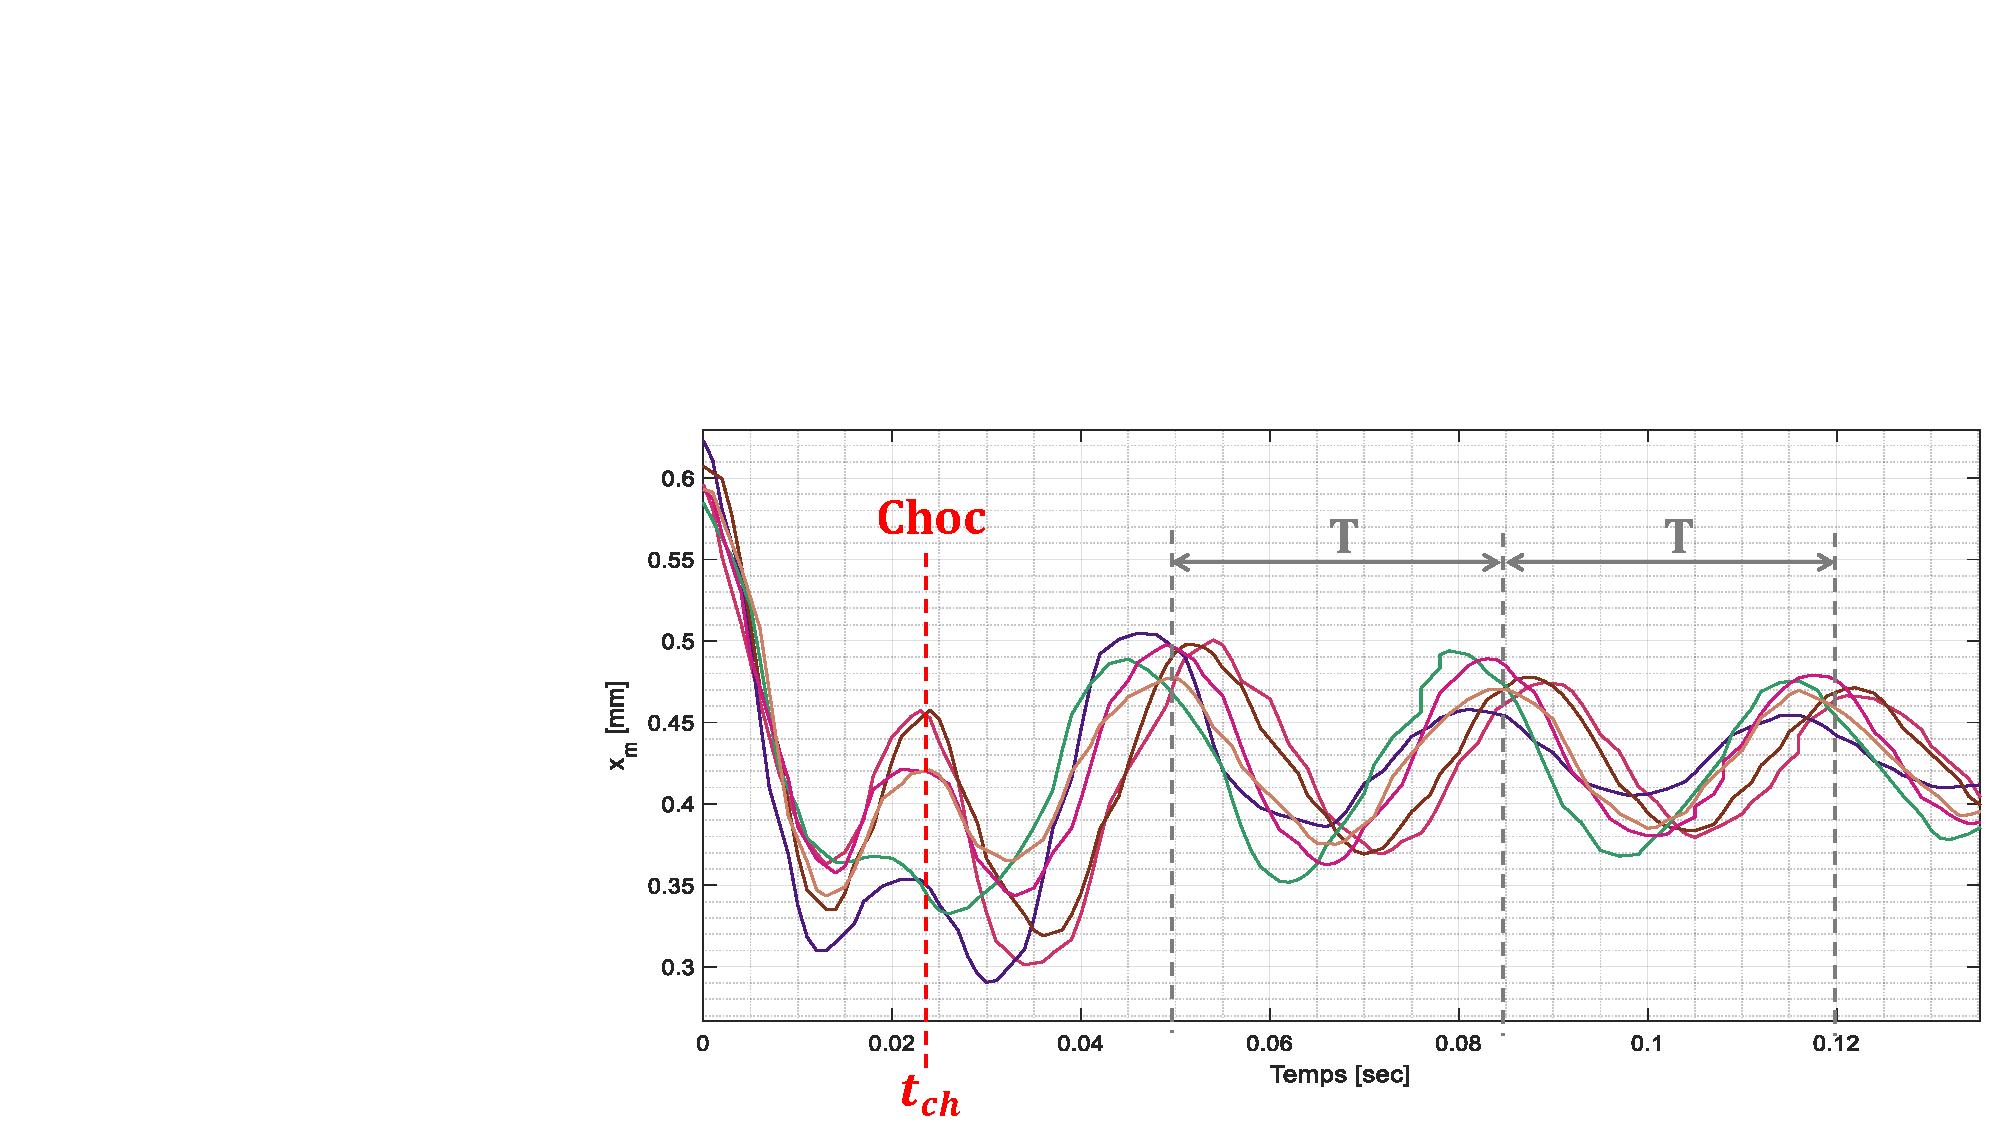
\includegraphics[trim={10cm 0cm 0cm 7cm},clip,width=\textwidth]{../Chap6/Figure/lachers_avec_tube_CHOC.pdf}
		\caption{Superposition de six lâchers consécutifs sur un système OBVH avec $a<1$mm}
		\label{fig:lachers_avec_tube_CHOC}
\end{center}	
\end{figure}    
%%%%%%%%%%%%%%%%%%%%%%%%%%%%%%%%%%%%	 

D'autre part, il a été constaté que le vieillissement des prototypes de VH a une influence sur leur fonctionnement. À des fins de manipulations sécurisées, nous avons opté pour l'utilisation d'huile végétale de tournesol pour le fonctionnement des composants hydrauliques. De plus, en remplacement de l'eau, cela permet de préserver les composants hydrauliques d'une oxydation prématurée. Aussi, l'huile offre une étanchéité capillaire aux déplaceurs des pistons hydrauliques par sa viscosité. En revanche, soumis au temps et à l'oxygène, l'huile végétale se polymérise et finit par durcir en un matériau gélatineux dont les propriétés mécaniques s'approchent de celles du silicone. La VH remplie d'huile végétale finit alors par être obstruée par un matériau très visqueux qui absorbe les oscillations de M, réduisant d'autant plus le rendement de conversion. À terme, tout l'énergie apportée par M pourrait être absorbée dans la VH. 

Une alternative à l'huile végétale pourrait alors être l'huile minérale. Les applications souhaitées étant médicales, il faudra privilégier des solutions bio-compatibles. De ce fait, les huiles synthétiques ne pourront pas faire partie des choix envisageables. Les joints d’étanchéité des composants hydrauliques devront par ailleurs être étudiés en conséquence, pour prévenir la corrosion par les huiles minérales.

De plus, la masse et l'éventuelle raideur supplémentaire de la portion de circuit hydraulique, devant aller depuis la partie mobile de la VH jusqu'au piston, n'a pas été considérée durant les essais. Le prototype d'OB a en effet été conçu pour une instrumentation complète autour du fonctionnement de celui-ci seul. L'ajout des VH est complexe au vu de l'encombrement du dispositif, s'il fallait en addition considérer la partie mobile du circuit hydraulique. Néanmoins, il serait possible d'envisager l'utilisation de liaison hydraulique constituée d'un tube souple en spirale partant de la partie mobile de la VH et se logeant dans le PH. En faisant varier le diamètre de la spirale, sa longueur, ainsi que le matériau, il serait envisageable de minimiser son influence sur la raideur supplémentaire ajoutée au système. La masse du circuit hydraulique en mouvement s'ajoutera à $m$ et devra être quantifiée pour dimensionner le convertisseur électromécanique.
   %///////////////////////////////////////////// 	
   \subsection{Pistes d'améliorations du modèle global}
   \label{subsec:6.4.2}
   %///////////////////////////////////////////// 
		%**********************************
		\subsubsection{Le modèle global}
		\label{subsec:6.4.2.a}
		%**********************************
Le modèle analytique global, corrélé avec les données expérimentales, prend en compte une majorité des éléments physiques pour rester fidèle avec la réalité. Malgré une dégradation de ses performances à l'issue de la fabrication et du montage, son comportement expérimental s'est révélé fidèle au modèle analytique. D'autres phénomènes peuvent par ailleurs être considérés dans le modèle afin d'améliorer sa capacité prédictive : 

\paragraph{Les stoppers de PHs.}
La résolution des équations modélisant la dynamique des différentes phases de fonctionnement se fait indépendamment dans le modèle numérique global. Les résultats des simulations présentés sur les figures \ref{fig:simu_pos_debit_Cf_pression_1CYCLE} et \ref{fig:simu_pos_Up_puissances_energie_1CYCLE} sont issus de la concaténation temporelle des variables de sortie des différents sous-systèmes indépendants. Certains scénarios ne sont alors pas considérés dans la résolution des modèles car l'intégration de ces éléments est trop complexe par la physique qui les définit, mais aussi par la manière dont le modèle à été programmé. Par exemple, la collision probable entre le piston inactif et la masse oscillante au moment du lâcher n'est pas programmée. Pour parer cela, nous avons considéré que le système est défaillant lorsque les positions respectives du piston passif et de la masse se rencontrent. Après avoir défini l'influence des différents paramètres sur le système global (tab. \ref{tab:influence parametres} et \ref{tab:influence parametres (suite)}), un réglage sur le paramètre adéquat permet d'éviter ce scénario. Néanmoins, il serait préférable d'intégrer une butée de fin de course sur les pistons, afin qu'ils évitent d'entraver le mouvement oscillatoire de la masse. Les répercutions de cette butée sur le circuit hydraulique devront aussi être prises en considération.

\paragraph*{Le contact PH-M.} L'actionnement hydraulique est considérée quasi-statique devant la fréquence des oscillations de la masse. Cette dernière est cependant à l'arrêt avant le premier contact avec le piston. Il serait alors intéressant d'intégrer un modèle de choc entre les deux composants afin d'étudier le comportement dynamique de la masse, ainsi que la réponse en pression du circuit hydraulique.

\paragraph{La variabilité de l'allure de la source hydraulique.}
L'allure de débit imposée (fig. \ref{fig:debit_ear}) est issue d'une ouverture et d'une fermeture complète de la mâchoire. Un mouvement partiel d'ouverture/fermeture pourrait aussi être envisagé dans le modèle, car il engendrerait alors des conditions initiales différentes pour un cycle de mastication complet qui suit. 
		%**********************************
		\subsubsection{Le circuit hydraulique}
		\label{subsec:6.4.2.b}
		%**********************************
Le comportement pression/débit du bouchon d'oreille, face à l'impédance mécanique de l'OB, n'a pas été expérimentalement caractérisée sur un sujet humain. La résolution complète du modèle dépend en effet de l'allure du débit et du volume maximal déplacé depuis l'oreille. La source n'admet, dans notre étude, aucune variabilité entre deux cycles de mastication. La robustesse de la prédiction théorique pourrait donc être améliorée avec l'intégration d'une courbe de caractérisation pression/volume du bouchon d'oreille soumis à l'impédance mécanique de l'OB.

Enfin, le fonctionnement du système est piloté par le comportement des VH. Nous avons présenté, dans le chapitre \ref{ch:4_Valves hydrauliques a base de tubes flexibles flambes}, des essais de caractérisation sur un seul prototype de VH fabriqué de façon artisanale par le biais de deux adaptateurs de diamètres. Le comportement hydraulique de la valve a été extrait en estimant de façon pragmatique les pertes de charges des irrégularités de fabrication lors des essais à $\theta=0$ (sec. \ref{sec:4.4_Caractérisations hydrauliques}). En prenant du recul, il est possible d'améliorer la robustesse des données expérimentales avec les considérations suivantes:
\begin{itemize}[label=$\circ$]
	\item Répéter le protocole d'essais sur plusieurs échantillons de VH et étudier expérimentalement l'influence du diamètre initial du tube.
 	\item Éviter toute adaptation de diamètre interne sur l'échantillon de VH pour se défaire de la majorité des irrégularités amenées par la fabrication.
 	 \item Augmenter les incréments d'angle et utiliser plusieurs gammes de capteurs de pression afin de garder une incertitude faible sur les mesures dans un ordre de grandeur de pression de travail donné.
\end{itemize} 
Le banc de test hydraulique instrumenté présenté sur la figure \ref{fig:essais_hydraulique_VH} peut s'adapter à différents diamètres de gaines rigides et de tubes Kapton pour se prêter à une étude complète de caractérisation des VH à base de tubes flambés avec les considérations introduites ci-dessus.
		%**********************************
		\subsubsection{Efficacité du système}
		\label{subsec:6.4.2.b}
		%**********************************
Le rendement théorique du système global a été estimé à 67.1\% lors de la phase de pré-dimensionnement, avec un rendement de 79\% pour l'OB seul (tab. \ref{tab:parametres électromécaniques} et \ref{tab:parametres_lacher_free}). Les corrélations modèle-essais, réalisées avec les données des caractérisations expérimentales de l'OB (ch. \ref{ch:3_Conception et fabrication du convertisseur electromecanique : OB + GPA}), des VH (ch. \ref{ch:4_Valves hydrauliques a base de tubes flexibles flambes}) et du contact M-VH (sous-sec. \ref{subsec:6.2.2_Essais de lacher experimentaux de M avec et sans VH}), ont permis de mettre en évidence les difficultés de réalisation du récupérateur. Les performances du convertisseur électromécanique diminuent jusqu'à un rendement de 2.6\% avec les considérations expérimentales (tab. \ref{tab:parametres lacher tube}).

Une grande partie de cette baisse est causée par la dégradation structurelle subie par l'OB durant sa fabrication et sa manipulation. Ces-derniers ont engendré une baisse de $84\%$ sur le rendement de l'OB (tab. \ref{tab:parametres_lacher_free}). Cela pourrait être évité en optant pour une méthode de dimensionnement différente. La raideur en rotation $K_{\varphi}$ des liaisons pivots a en effet été calculée pour limiter les contraintes de flexion des LF. La géométrie résultante a donné lieu à des épaisseurs de lames de $75$µm avec un coefficient de sécurité de 6 sur la limite élastique du matériau, sur la plage d'angle $\varphi$ d'utilisation envisagée. Le retour sur expérience suggère qu'une épaisseur si faible dégrade nettement la transmission d'effort en compression des LF vers le GPA. Il serait donc judicieux de revoir le dimensionnement de l'OB de façon à augmenter sa résistance structurelle face aux sollicitations mécaniques externes et internes. L’élément dimensionnant devrait alors être la pré-contrainte admissible par le GPA au passage de la masse par la position $x_m=0$ qui, pour le GPA utilisé, a été calculée à $F_{adm}=18$N avec la documentation technique du dispositif (ann. \ref{Ann:6_Documentation technique sur l'APA50XS Cedrat Technologies}). Ainsi, il pourrait être envisageable d'utiliser des épaisseurs de LF supérieures à 200µm, soit plus de deux fois plus que le cas présent.

L'autre majeure partie de l'énergie dissipée est due au frottement sec entre la masse et la VH. Des pistes d'améliorations sur cet aspect ont été introduites plus tôt dans cette section. Le coefficient de frottement entre les deux solides a été estimé à $\micro_{fs}=0.42$ et reste cohérent avec les valeurs estimées dans la littérature pour le frottement non lubrifié entre un polymère et un métal \cite{Nosonovsky2013}. Ce dernier peut être réduit de près de 90\% si le teflon est utilisé comme interface de contact entre les deux composants\cite{Nosonovsky2013}. Si, de surcroît, la masse est équipée d'un roulement, la réduction des frottement pourrait être d'autant plus intéressante.

Enfin, le rendement global du système est dépendant des paramètres qui ont été listés dans les tableaux \ref{tab:influence parametres} et \ref{tab:influence parametres (suite)} avec leurs influences respectives sur le système. La complexité du couplage entre les différents paramètres se traduit par la proportionnalité inverse de leur influence sur le critère de rendement et celui de fonctionnement. en effet, une simple modification améliorant théoriquement le rendement du système peut engendrer un défaut de fonctionnement dans ce-dernier ($r_{Cf}<10$ ou oscillateur monostable car $K_{VH}$ trop importante).  Un compromis est alors à trouver pour maximiser le rendement et garantir le fonctionnement du système. Un travail à faire en perspectives serait alors de dresser un plan d'expérience avec ces paramètres, pour élaborer un algorithme capable d'optimiser les réglages du système pour une entrée énergétique donnée.






% %%%%%%%%%%%%%%%%%
% \begin{table}[!htbp]
% 	\begin{minipage}{0.32\textwidth}
% 	\centering
% 	\rowcolors[]{2}{black!8}{}{
% 		\begin{tabular}{ l | c }
% \rowcolor{blue!10}    
% \hline
% \rowcolor{blue!10}    
% Définition & Symbole	\\ 
% \hline
% Pression de confort 			& $p_c$ 				\\
% Cylindrée bouchon d'oreille 	& $\Delta V_{ear,m}$	\\       
% Cylindrée bouchon d'oreille 	& $\Delta V_{ear,m}$	\\                
% \hline           
% 		\end{tabular}}
% 		\caption{Paramètres source}
%         \label{tab:parametres_source}
% \end{minipage}	
% \hfillx
% \begin{minipage}{0.32\textwidth}
% 	\centering
% 	\rowcolors[]{2}{black!8}{}{
% 		\begin{tabular}{ c | c }
% \rowcolor{blue!10}    
% \hline
% \rowcolor{blue!10}    
% Définition & Symbole	\\ 
% \hline
% Pression de confort 			& $p_c$ 				\\
% Cylindrée bouchon d'oreille 	& $\Delta V_{ear,m}$	\\       
% Cylindrée bouchon d'oreille 	& $\Delta V_{ear,m}$	\\                
% \hline           
% 		\end{tabular}}
% 		\caption{Paramètres de dimensionnement}
%         \label{tab:parametres_dimensionnement}
% \end{minipage}
% \hfillx
% \begin{minipage}{0.32\textwidth}
% 	\centering
% 	\rowcolors[]{2}{black!8}{}{
% 		\begin{tabular}{ c | c }
% \rowcolor{blue!10}    
% \hline
% \rowcolor{blue!10}    
% Définition & Symbole	\\ 
% \hline
% Pression de confort 			& $p_c$ 				\\
% Cylindrée bouchon d'oreille 	& $\Delta V_{ear,m}$	\\       
% Cylindrée bouchon d'oreille 	& $\Delta V_{ear,m}$	\\                
% \hline           
% 		\end{tabular}}
% 		\caption{Paramètres de fonctionnement}
%         \label{tab:parametres_dimensionnement}
% \end{minipage}	
% \end{table} 
% %%%%%%%%%%%%%%%%%%%%%  


% L'implémentation du comportement expérimental statique et hydraulique de la VH, ainsi que les frottements générés au contact M-VH, influent sur la dynamique du système global. En utilisant le modèle système global établi dans la section \ref{sec:2.5_Simulations et dimensionnement préliminaire du système de récupération} et, corrigé avec les donées expérimentales, nous pouvons simuler le comportement du système global. Il n'a pas été développé d'algorithme d'optimisation des différents paramètres pour un fonctionnement maximisant le rendement de conversion d'énergie pour un CDC énergétique donné. Nous avons cependant pu établir la tendance d'évolution de ce dernier en fonction de l'évolution des paramètres du système. 

% fabriquée à partir du tube T100p dans modèle système défini à la section \ref{sec:2.5_Simulations et dimensionnement préliminaire du système de récupération}, on peut résoudre de façon numérique l'évolution des paramètres du systèmes OBVH$_{eq}$ redimensionné.
% En nous appuyant sur les données issues des essais expérimentaux statiques sur le tube T100p, nous pouvons recaler les paramètres dy stsème OBVH afin de générer le nouveau jeu de paramètres du modèle OBVH$_{xp}$.\\
% Comme pour le modèle OBVH$_{eq}$ implémentant l'impact du comportement théorique du tube T40, nous devons nous fixer une plage d'angle d'utilisation pour le tube T100p. Plusieurs choix sont possibles, comme on a pu voir précédemment et les critères de sélection restent les mêmes. Nous devons donc une nouvelle fois trouver un compromis sur la plage d'angle où :
% \begin{itemize}
% 	\item L'impact de $K_{VH}$ n'induit pas un flambement à vide $\tilde{x_{0}}_{,xp}$ supérieur à $x_{0,m}$ défini à l'équation \ref{eq:x_0m}, afin d'assurer un meilleur couplage électromécanique et sauvegarder l'intégrité structurelle de l'OB 
% 	\item Le coefficient de PdC $Cf_{VH}({\theta_0})$ dans la valve ouverte est minimal pour maximiser le rendement du système global. 
% \end{itemize}	 
% Pour se fixer un point de départ, on se propose de comparer l'allure de la perte de charge de la VH T40 théorique, et celle du T100p. On peut voir alors sur la figure \ref{fig:(Cf_VH)_vs_theta_T40theo_T100exp} la superposition de $Cf_{VH}$ pour ces deux cas.
% %%%%%%%%%%%%%%%%%%%%%%%%%
% \begin{figure}[!htbp]
% \begin{center}
% 	\begin{subfigure}[b]{0.48\textwidth}
%     	\captionsetup{justification=centering}
% 	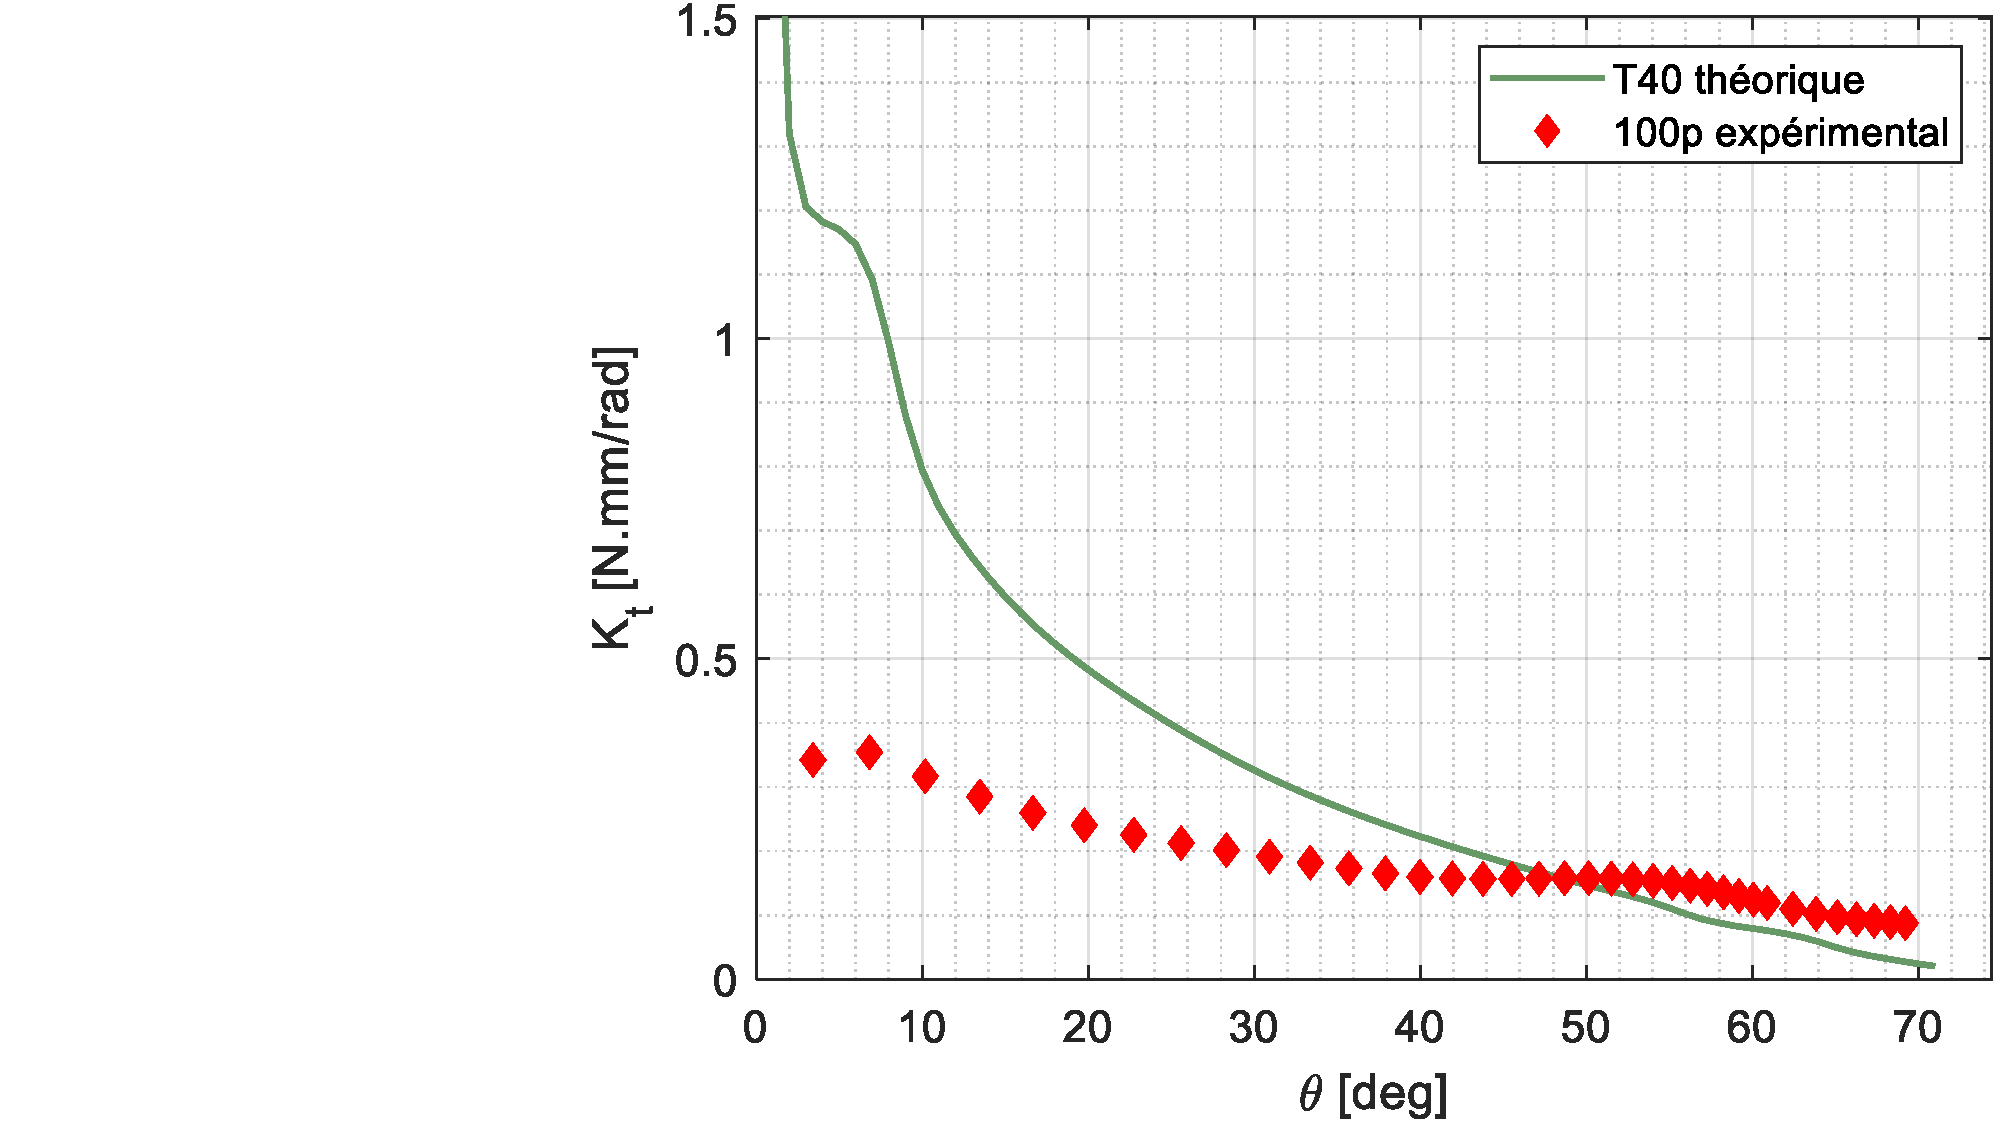
\includegraphics[trim={10cm 0cm 0cm 0cm},clip, 					                 width=\textwidth]{../Chap5/Figure/(K_VH)_vs_theta_T40theo_T100exp_essai2.pdf}
% 	\caption{$K_{VH}$}
% 	\label{fig:(K_VH)_vs_theta_T40theo_T100exp}
% 	\end{subfigure}
% \hfillx
% 	\begin{subfigure}[b]{0.48\textwidth}
%     	\captionsetup{justification=centering}
% 	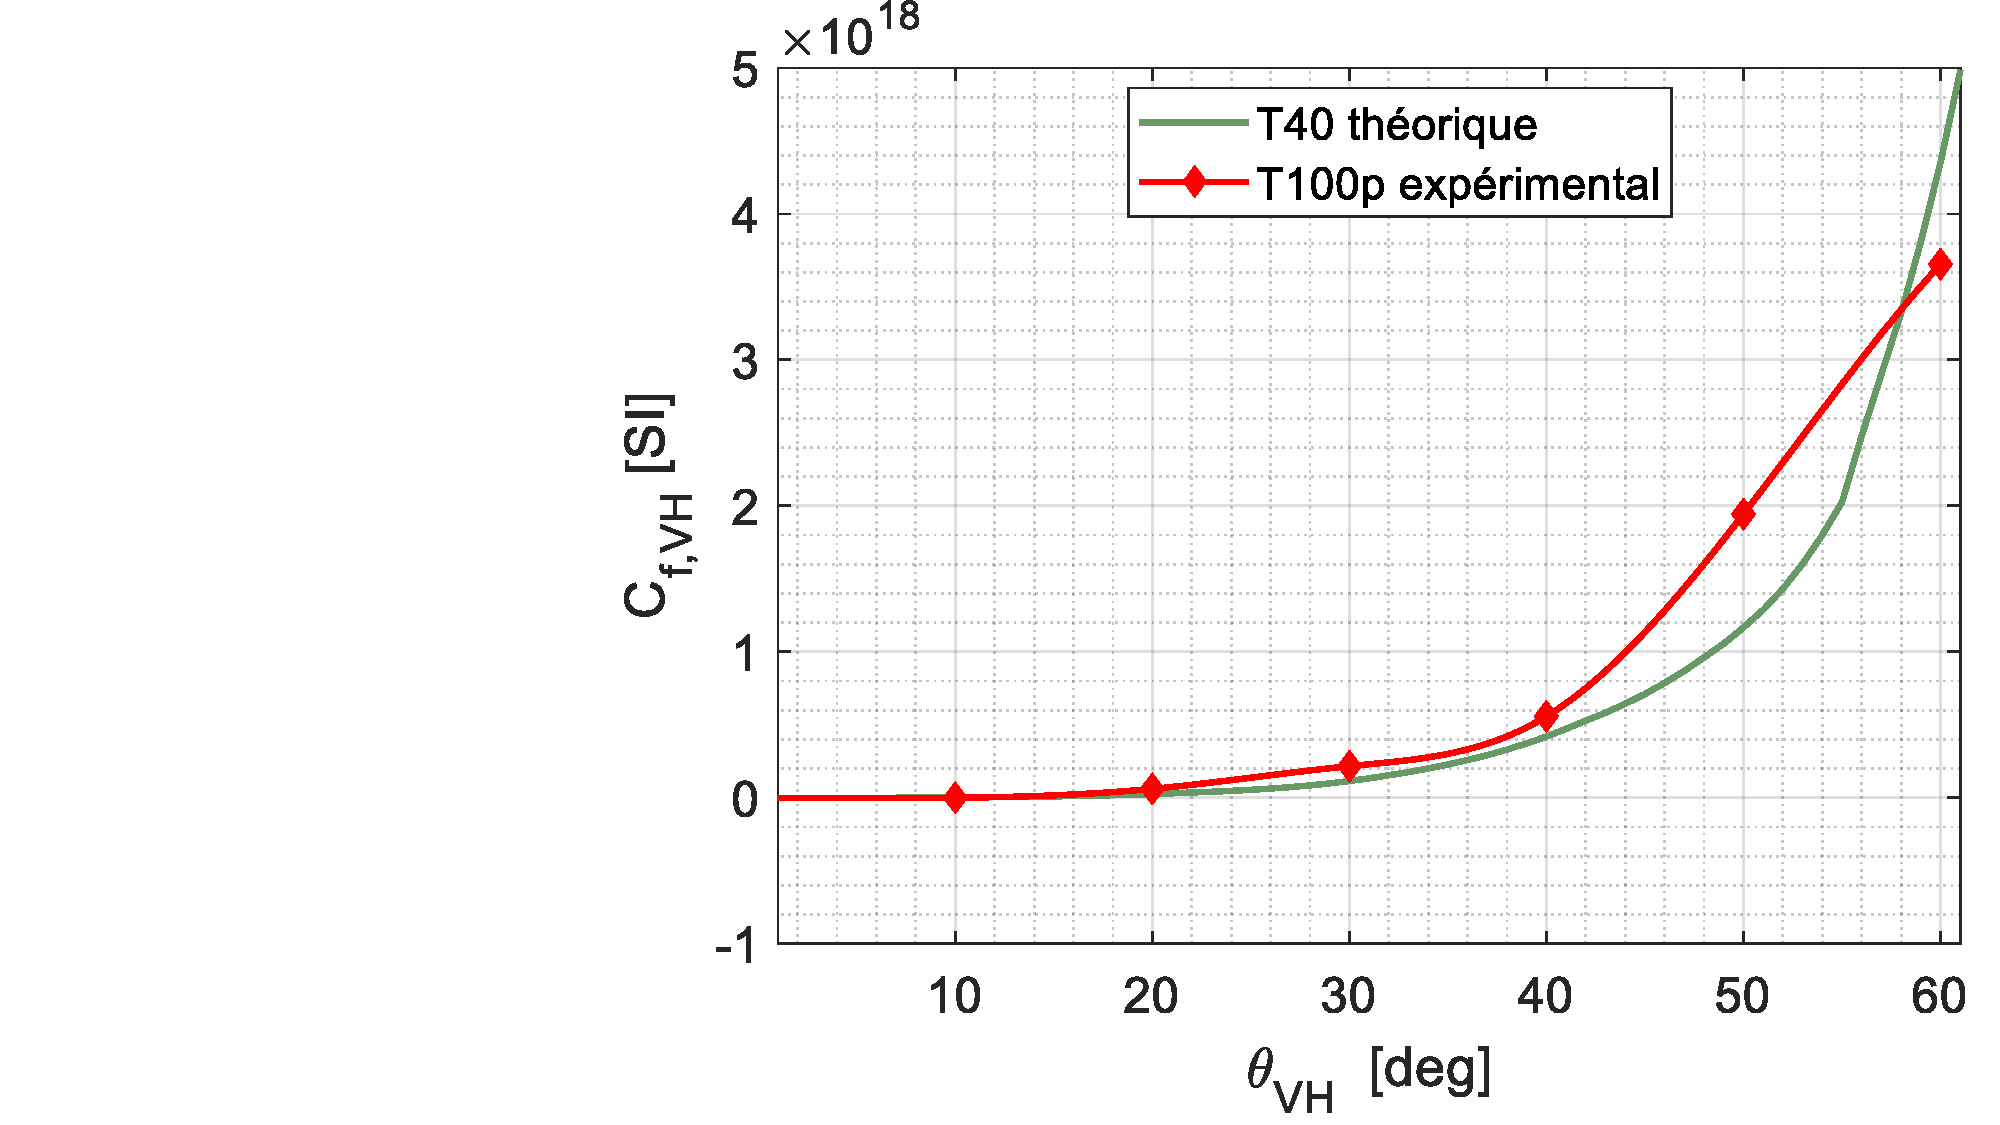
\includegraphics[trim={10cm 0cm 0cm 0cm},clip, 					                 width=\textwidth]{../Chap5/Figure/(Cf_VH)_vs_theta_T40theo_T100exp.pdf}
% 	\caption{$Cf_{VH}$}
% 	\label{fig:(Cf_VH)_vs_theta_T40theo_T100exp} 
% 	\end{subfigure}
% 	\caption{Comparaison de $K_{VH}$ et $Cf_{VH}$ pour le modèle théorique du tube T40 et les données expérimentales du tube T100p}
% 	\label{fig:Cf_comparaison_theorie_experimental}
% \end{center}	
% \end{figure}
% %%%%%%%%%%%%%%%%
% On constate que le comportement mécanique et hydraulique dans les deux jeux de données est du même ordre de grandeur et garde les mêmes tendances. Une chose cependant à noter est que l'étranglement du tube T100p semble se faire plus rapidement avec la flexion, pour les angles inférieurs à \ang{58}. On se donne donc comme angle de départ $\theta_0=\ang{20}$, légèrement plus faible que pour le T40 théorique car le T100p expérimental est plus souple.\\
% Pour dimensionner l'OBVH$_{xp}$ à des fins de simulations, nous allons comme précédemment majorer la rigidité du tube par sa valeur à $\theta_0$, valant $K_{T100}(\ang{20})\approx 4$Nmm/rad. Sur le volet hydraulique, nous allons nous caler sur la plage d'angle $\Delta \theta_{20,45}$ aussi large que précédemment car on observe une évolution similaire de $Cf_{VH}$ entre les deux tubes. Le rapport de fermeture $r_{cf,xp}=18$ et est, lui aussi, très similaire au rapport $r_{cf,eq}=17$ du modèle OBVH$_{eq}$. Nous pouvons alors calculer les paramètres de l'OBVH$_{xp}$ avec le système d'équations \ref{eq:x0_eq}. Les résultats des calculs de redimensionnement sont listés dans le teableau \ref{tab:recalage_OBVH_xp}, en parallèle avec ceux du modèle précédent.\\	
% 	Afin d'implémenter le comportement hydraulique du tube T100p dans la simulation système, il nous est nécessaire d'avoir des points intermédiaires entre les angles où les essais ont été réalisés. Pour ce faire nous avons appliqué une interpolation cubique sur le jeu de données expérimentales pour $Cf_{VH}$ et intégré au programme Simulink chargé de résoudre les équations différentielles régissant le comportement du système global.\\
% %%%%%%%%%%%%%%%%%%%%%%%%%%%%%%%%%%%%	
% \begin{figure}[!htb]
% \begin{center}
%     \captionsetup{justification=centering} 
% 	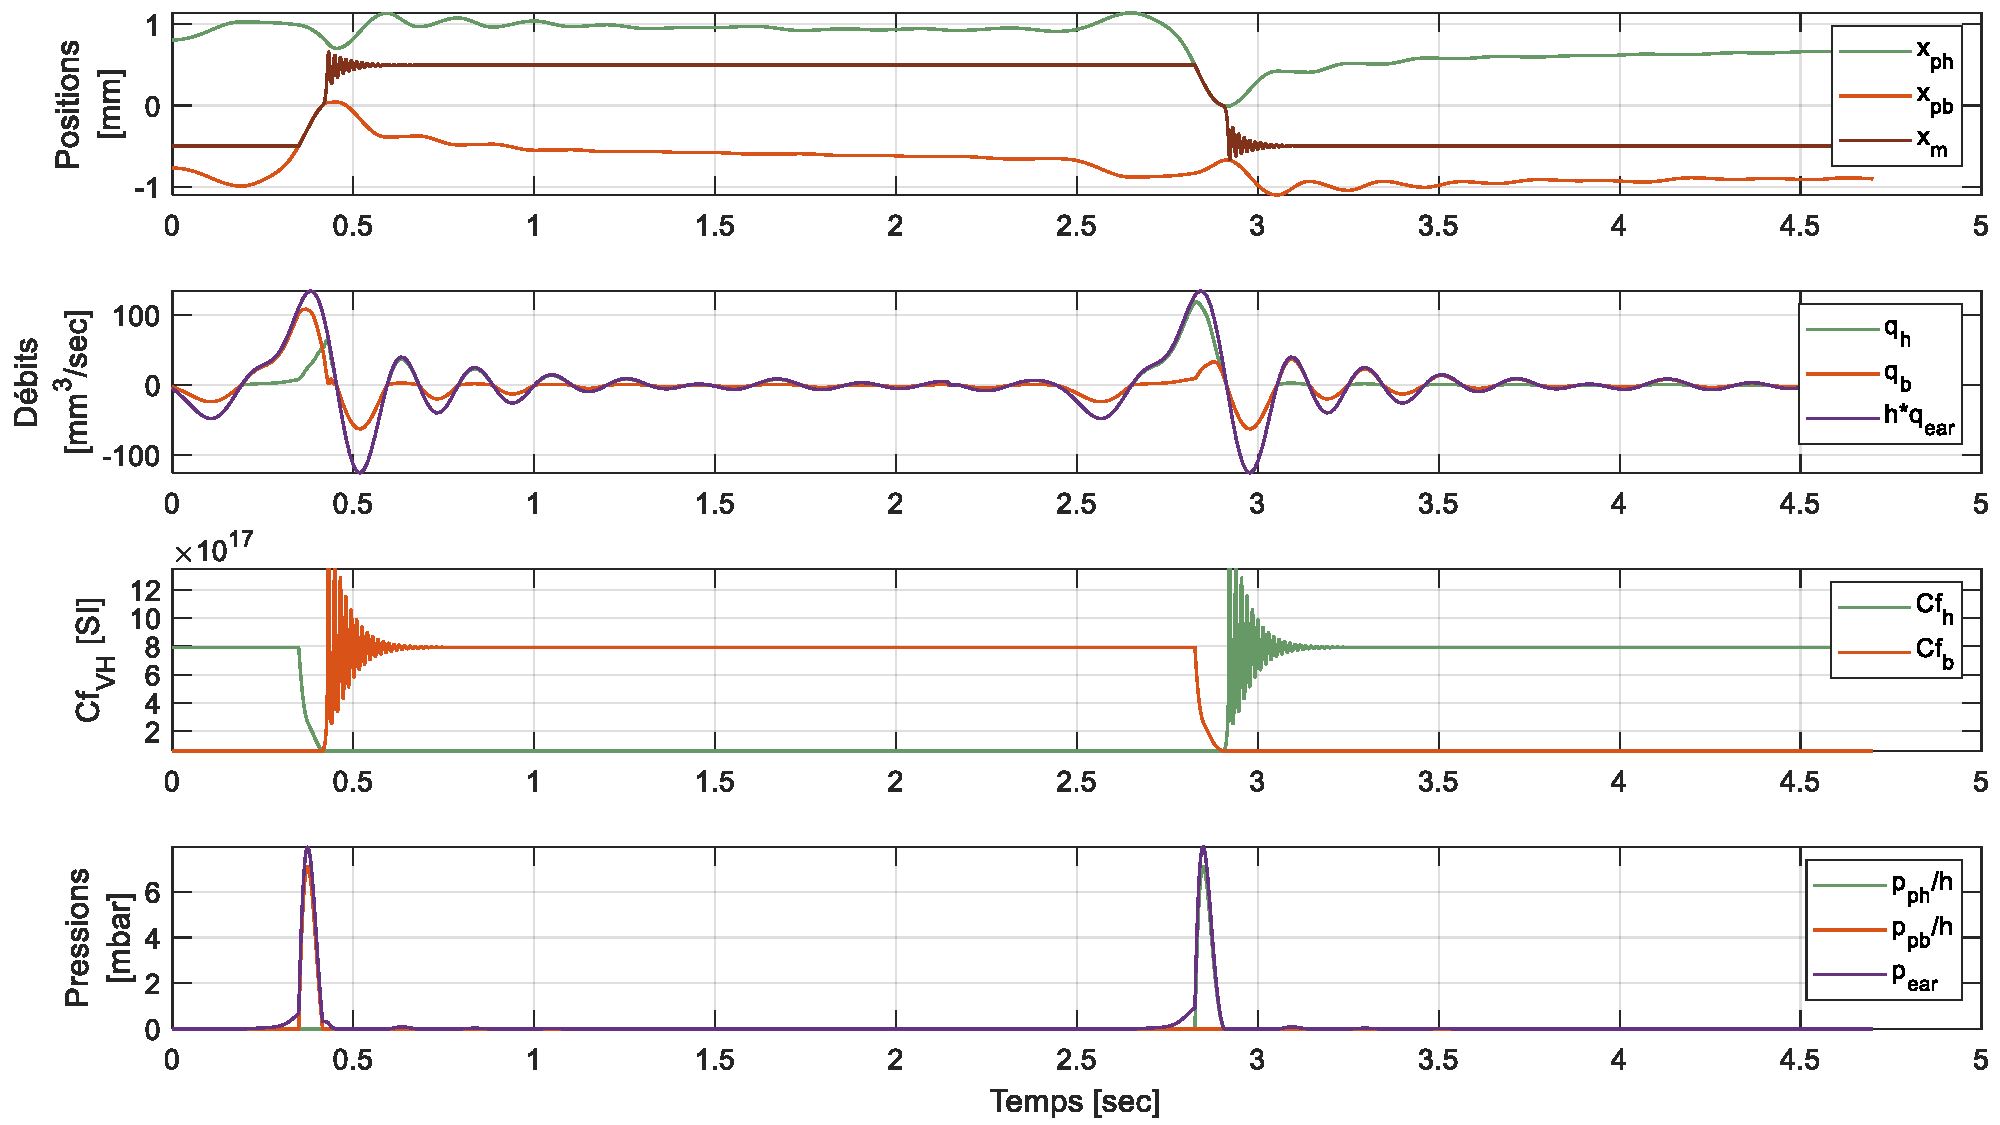
\includegraphics[trim={0cm 0cm 0cm 0cm},clip, 					                 width=\textwidth]{../Chap5/Figure/simulink_OBVHexp__position_debit_Cf_pression_2CYCLES.pdf}
% 	\caption{Résultats de simulation pour les positions, débits, coefficients de PdC et pressions en concordance de temps - 1 cycle avec $K_{T100p}(\ang{20})$}
% 	\label{fig:simulink_OBVHexp__position_debit_Cf_pression_2CYCLES}
% \end{center}	
% \end{figure}    
% %%%%%%%%%%%%%%%%%%%%%%%%%%%%%%%%%%%% 
% %%%%%%%%%%%%%%%%%%%%%%%%%%%%%%%%%%%%	
% \begin{figure}[!htb]
% \begin{center}
%     \captionsetup{justification=centering} 
% 	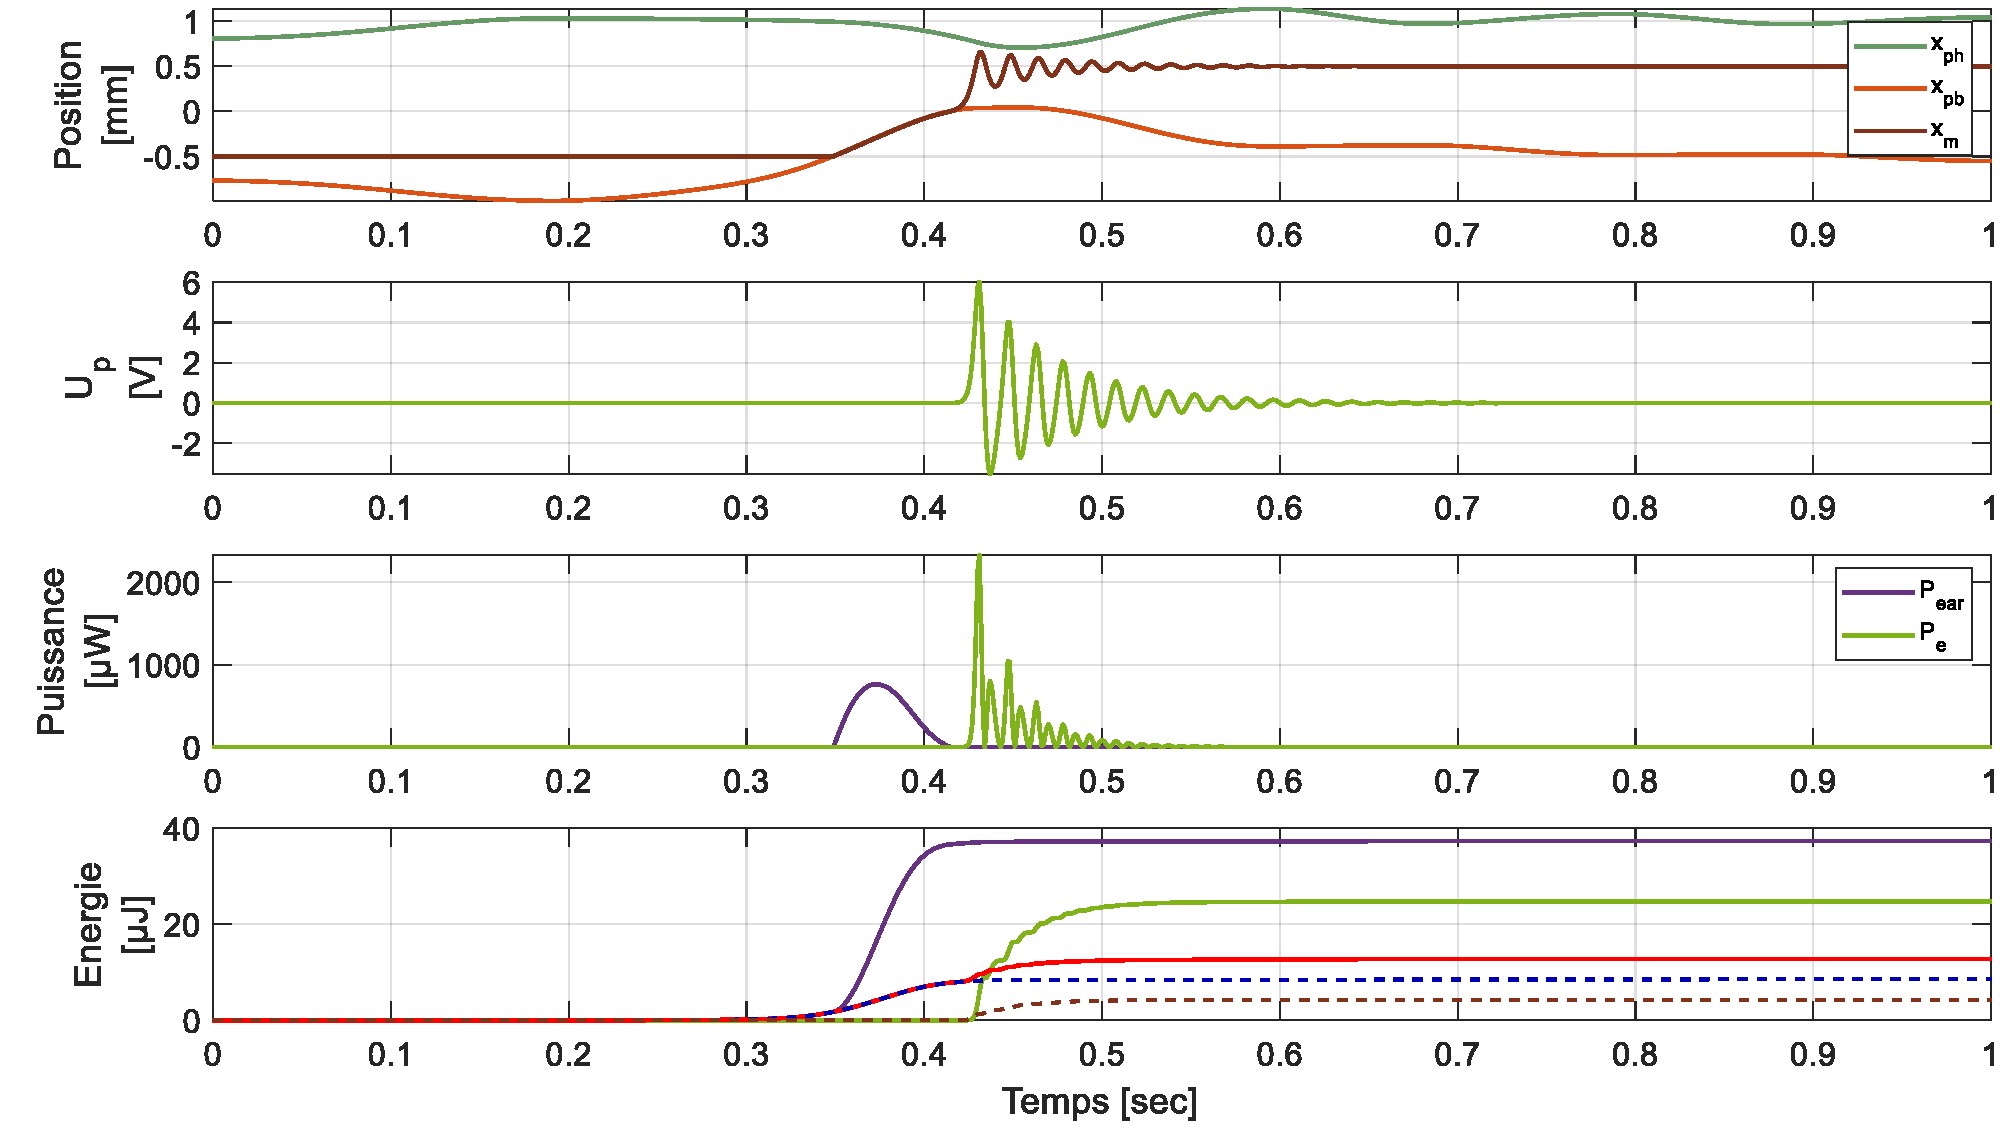
\includegraphics[trim={0cm 0cm 0cm 0cm},clip, 					                 width=\textwidth]{../Chap5/Figure/simulink_OBVHeq__position_Up_puissance_energie_1CYCLE.pdf}
% 	\caption{Résultats de simulation pour les positions, tension GPA, puissances et énergies - 1 cycle avec $K_{T100p}(\ang{20})$}
% 	\label{fig:simulink_OBVHeq__position_Up_puissance_energie_1CYCLE}
% \end{center}	
% \end{figure}    
% %%%%%%%%%%%%%%%%%%%%%%%%%%%%%%%%%%%% 
% Les résultats de simulation système du modèle OBVH$_{xp}$ implémentant les données expérimentales du comportement du tube T100p sur la plage d'angle $\Delta\theta_{20,45}$ apparaissent sur les figures \ref{fig:simulink_OBVHexp__position_debit_Cf_pression_2CYCLES} et \ref{fig:simulink_OBVHeq__position_Up_puissance_energie_1CYCLE}. Le faible écart de rigidité entre les deux tubes induit un comportement mécanique similaire au modèle OBVH$_{es}$. En revanche, on peut voir sur la figure \ref{fig:comparaison_Cfcdc_CfT40_Cf_T100p} que le comportement hydraulique est légèrement différent. En effet, la valve T100p expérimentale se ferme plus rapidement que la valve T40 théorique. Aussi, comme on le voit dans le tableau des paramètres, les PdC sont légèrement plus importantes dans la valve ouverte T100p et donc on y dissipe plus d'énergie pour faire passer le même débit. Ceci explique la légère baisse de rendement constatée dans ce nouveau modèle, en comparaison à l'ancien.\\
% %%%%%%%%%%%%%%%%%%%%%%%%%%%%%%%%%%%%	
% \begin{figure}[!htb]
% \begin{center}
%     \captionsetup{justification=centering} 
% 	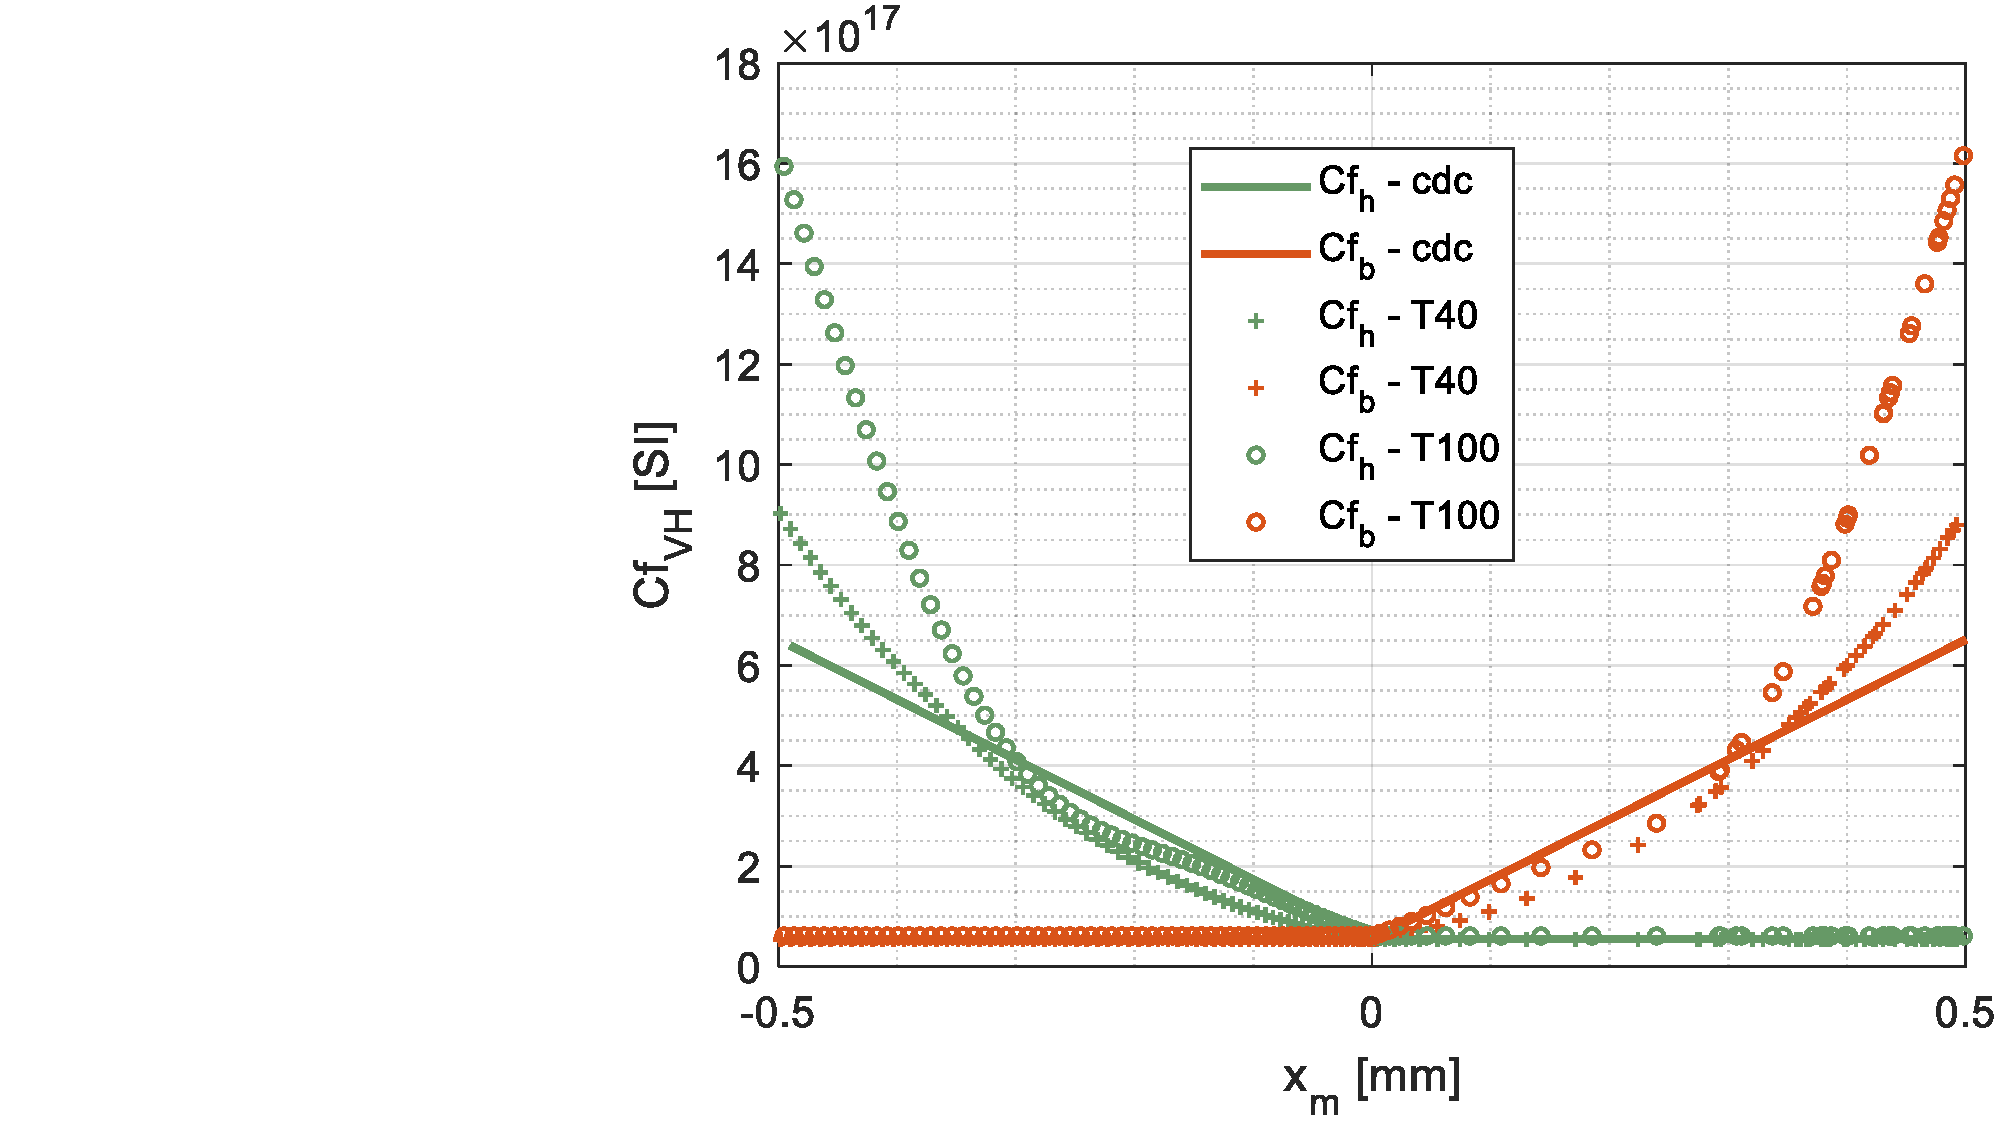
\includegraphics[trim={10cm 0cm 0cm 0cm},clip, 					                 width=0.6\textwidth]{../Chap5/Figure/comparaison_Cfcdc_Cfvh_Cfexp.pdf}
% 	\caption{Comparaison $Cf_{VH}(x_m)$ pour le cdc, le tube T40 théorique et T100p expérimental}
% 	\label{fig:comparaison_Cfcdc_CfT40_Cf_T100p}
% \end{center}	
% \end{figure}    
% %%%%%%%%%%%%%%%%%%%%%%%%%%%%%%%%%%%% 
% On notera ici que le dimensionnement a été fait de façon à se placer sur la limite optimale de tous les paramètres, permettant un rendement maximal et un cyclage effectif de M sur deux fermetures de mâchoire. En réalité, un léger écart sur les paramètres listés dans le tableau \ref{tab:recalage_OBVH_xp} induirait un comportement différent sur le système. Nous avons exprimé les critères qui nous ont amené à dimensionner le système de la sorte, mais nous savons qu'expérimentalement il est probable que nous ayons besoin d'ajuster les paramètres avec des coefficients de sécurité permettant de compenser les erreurs de réglage manuels et les imperfections de fabrication et de montage.